\documentclass[article]{elsarticle}

\usepackage{lineno,hyperref}
\modulolinenumbers[5]

%% Nomenclature divided into different sections
\usepackage{framed}
\usepackage{mdframed}
\mdfdefinestyle{mdfexample1}{innerleftmargin=1cm,innerrightmargin=1cm,roundcorner=10pt,innertopmargin = 5pt, innerbottommargin = 5pt}

\usepackage{multicol} 
\usepackage[nonumberlist,nopostdot,nomain,automake]{glossaries}
\newglossary{v}{vas}{vao}{Variables}
\newglossary{s}{ses}{seo}{Sets}
\newglossary{p}{pas}{pao}{Parameters}
\newglossary{a}{aas}{aao}{Abbreviations}
\makeglossaries

%% Variables
\newglossaryentry{v1}{name =\ensuremath{CF_{t,s}}, description = {Fuel costs in year $t$ by ship $s$},type= v}
\newglossaryentry{v2}{name =\ensuremath{CI_{t,s}}, description = {Infrastructure costs in year $t$ by ship $s$},type= v}
\newglossaryentry{v3}{name =\ensuremath{CS_{t,s}}, description = {Ship costs in year $t$ by ship $s$},type= v}
\newglossaryentry{v4}{name =\ensuremath{fa_{t,s}}, description = {Fuel amount in year $t$ by ship $s$},type= v}
\newglossaryentry{v5}{name =\ensuremath{EC_{t,s}}, description = {CO$_2$ emissions in year $t$ by ship $s$},type= v}
\newglossaryentry{v6}{name =\ensuremath{EM_{t,s}}, description = {CH$_4$ emissions in year $t$ by ship $s$},type= v}
\newglossaryentry{v7}{name =\ensuremath{fainit_{t,s}}, description = {Initial fuel amount in year $t$ by ship $s$},type= v}
\newglossaryentry{v8}{name =\ensuremath{faicap_{t,s}}, description = {Infrastructure capacity in year $t$ by ship $s$},type= v}
\newglossaryentry{v9}{name =\ensuremath{fascap_{t,s}}, description = {Ship capacity in year $t$ by ship $s$},type= v}
\newglossaryentry{v10}{name =\ensuremath{faiup_{t,s}}, description = {Additional infrastructure capacity in year $t$ by ship $s$},type= v}
\newglossaryentry{v11}{name =\ensuremath{fasup_{t,s}}, description = {Additional ship capacity in year $t$ by ship $s$},type= v}

%% Sets
\newglossaryentry{s1}{name =\ensuremath{\mathcal{T}},description = {All time steps (years)},  type = s}
\newglossaryentry{s2}{name =\ensuremath{\mathcal{S}},description = {All ships},  type = s}
\newglossaryentry{s3}{name =\ensuremath{\mathcal{RO}(s)},description = {Refit option per ship type s},  type = s}
\newglossaryentry{s4}{name =\ensuremath{\mathcal{SNG}},description = {Ships not global-SECAs compliant},  type = s}
\newglossaryentry{s5}{name =\ensuremath{\mathcal{NT}},description = {Ships not NECAs compliant},  type = s}
\newglossaryentry{s6}{name =\ensuremath{\mathcal{SB}},description = {Ships burning bio-fuel},  type = s}
\newglossaryentry{s7}{name =\ensuremath{\mathcal{SR}},description = {Ships for short range},  type = s}
\newglossaryentry{s8}{name =\ensuremath{\mathcal{SNE}},description = {Ship not SECAs compliant},  type = s}


%% Parameters
\newglossaryentry{p1}{name =\ensuremath{cf_{t,s}},description={Fuel costs in year $t$ by ship $s$},type= p}
\newglossaryentry{p2}{name =\ensuremath{li_{t,s}},description={Infrastructure lifetime in year $t$ by ship $s$},type= p}
\newglossaryentry{p3}{name =\ensuremath{ci_{t,s}},description={Infrastructure costs in year $t$ by ship $s$},type= p}
\newglossaryentry{p4}{name =\ensuremath{ls_{t,s}},description={Ship lifetime in year $t$ by ship $s$},type= p}
\newglossaryentry{p5}{name =\ensuremath{cs_{t,s}},description={Ship costs in year $t$ by ship $s$},type= p}
\newglossaryentry{p6}{name =\ensuremath{ba_{t}},description={Bio-fuel availability in year $t$},type= p}
\newglossaryentry{p7}{name =\ensuremath{tdtotal_{t}},description={Total transport demand in year $t$},type= p}
\newglossaryentry{p8}{name =\ensuremath{tdshort_{t}},description={Transport demand on short range in year $t$},type= p}
\newglossaryentry{p9}{name =\ensuremath{tdnoneca_{t}},description={Transport demand outside ECAs in year $t$},type= p}
\newglossaryentry{p10}{name =\ensuremath{ts_{t,s}},description={Transport supply in year $t$ by ship $s$},type= p}
\newglossaryentry{p11}{name =\ensuremath{eb},description={Emission budget},type= p}
\newglossaryentry{p12}{name =\ensuremath{et},description={Emission target},type= p}
\newglossaryentry{p13}{name =\ensuremath{ec_{t,s}},description={CO$_2$ emissions in year $t$ by ship $s$},type= p}
\newglossaryentry{p14}{name =\ensuremath{em_{t,s}},description={CH$_4$ emissions in year $t$ by ship $s$},type= p}
\newglossaryentry{p15}{name =\ensuremath{slnonecayr},description={Inception year of global ECA},type= p}
\newglossaryentry{p16}{name =\ensuremath{tlecayr},description={Inception year of NECAs},type= p}

%% Abbreviations
\newglossaryentry{a1}{name = {ECA}, description={Emission control area},type= a}
\newglossaryentry{a2}{name = {SECA}, description={Sulphur emission control area},type= a}
\newglossaryentry{a3}{name = {NECA}, description={Nitrogen emission control area},type= a}

\usepackage{hyperref}
\makeatletter
\providecommand{\doi}[1]{%
  \begingroup
    \let\bibinfo\@secondoftwo
    \urlstyle{rm}%
    \href{http://dx.doi.org/#1}{%
      doi:\discretionary{}{}{}%
      \nolinkurl{#1}%
    }%
  \endgroup
}
\makeatother


\journal{Journal of \LaTeX\ Templates}

%% Additional packages
\usepackage{amsmath}
\usepackage{cleveref}
\usepackage{eurosym}
\usepackage{gensymb}
\usepackage{booktabs}
\usepackage{caption}


%%%%%%%%%%%%%%%%%%%%%%%
%% Elsevier bibliography styles
%%%%%%%%%%%%%%%%%%%%%%%
%% To change the style, put a % in front of the second line of the current style and
%% remove the % from the second line of the style you would like to use.
%%%%%%%%%%%%%%%%%%%%%%%

%% Numbered
%\bibliographystyle{model1-num-names}

%% Numbered without titles
%\bibliographystyle{model1a-num-names}

%% Harvard
%\bibliographystyle{model2-names.bst}\biboptions{authoryear}

%% Vancouver numbered
%\usepackage{numcompress}\bibliographystyle{model3-num-names}

%% Vancouver name/year
%\usepackage{numcompress}\bibliographystyle{model4-names}\biboptions{authoryear}

%% APA style
%\bibliographystyle{model5-names}\biboptions{authoryear}

%% AMA style
%\usepackage{numcompress}\bibliographystyle{model6-num-names}

%% `Elsevier LaTeX' style
\bibliographystyle{elsarticle-num-names}
%%%%%%%%%%%%%%%%%%%%%%%

\begin{document}

\begin{frontmatter}

\title{Future Marine Fuels - A Danish Case Study on Climate Compatible Energy Pathways}
%\tnotetext[mytitlenote]{Fully documented templates are available in the elsarticle package on %\href{http://www.ctan.org/tex-archive/macros/latex/contrib/elsarticle}{CTAN}.}

%% Group authors per affiliation:
\author[label1]{Till ben Brahim\corref{cor1}}
\address[label1]{Technical University of Denmark, Produktionstorvet, Bygning 426, 2800 Kongens Lyngby, Denmark}
\ead{tilseb@dtu.dk}

\cortext[cor1]{Corresponding author}

\author[label1]{Frauke Wiese}
\ead{frwi@dtu.dk}

\author[label1]{Marie Muenster}
\ead{maem@dtu.dk}

\begin{abstract}
% A concise and factual abstract is required. The abstract should state briefly the purpose of the research, the principal results and major conclusions. An abstract is often presented separately from the article, so it must be able to stand alone. For this reason, References should be avoided, but if essential, then cite the author(s) and year(s). Also, non-standard or uncommon abbreviations should be avoided, but if essential they must be defined at their first mention in the abstract itself.

% purpose of the research
The purpose of this research is the development of sustainable energy pathways for the Danish maritime cargo sector, which contribute to green house gas emission reductions by a fair share and finally become CO$_2$e-neutral in 2050. The achievement of carbon-neutrality in the shipping sector is of great importance for reaching the targets of the Paris Agreement.
% principal results
The modelling results indicate that either strong regulative carbon budgets or a carbon price of 350--450 \euro(2016)/t~CO$_2$e would be necessary to induce the urgent transition. This would double today's average cargo transport costs. However, the average import values would only increase by 6 to 8 \%.
Regarding fuel technologies, hydrogen, methanol and ammonia are from a socio-economic cost perspective most compatible. Though, due to high cost uncertainties there is no clear winner.
% major conclusions
Liquefied natural gas as an alternative intermediate solution would only have a short window of opportunity, mainly because of leakage problems of methane causing high greenhouse gas emissions as well as high fuel and technology costs. If this gaseous fuel is based on renewable sources, the so-called LBG can only play a role with drastically reduced methane leakage.

\vspace{2ex}

This research did not receive any specific grant from funding agencies in the public, commercial, or
not-for-profit sectors.
\end{abstract}

\begin{keyword}
% \texttt{elsarticle.cls}\sep \LaTeX\sep Elsevier \sep template
% \MSC[2010] 00-01\sep  99-00
Maritime transport\sep Marine fuels\sep Energy modelling\sep Emission reduction\sep Danish case-study 
\end{keyword}

\end{frontmatter}

\linenumbers

\section{Introduction}
% 1000
% The journal covers research in mechanical engineering and thermal sciences, with a strong focus on energy analysis, energy modelling and prediction, integrated energy systems, energy planning and energy management.

% What is required from the climate side and what does the IMO suggest so far
The ambition to reach climate pathways with limited overshoot of 1.5~\degree C requires global net zero CO$_2$ emissions by 2050 \cite{IPCC2018}. This implies a massive reduction of fossil fuels in the energy system. Several studies based on energy system models have shown possible pathways to net zero emissions for the electricity supply from country to continents and the whole world \cite{Climact2018} (TODO:references) and also for the heat sector. Although transport is more challenging \cite{Salvucci2018,Schafer2012} (TODO:cite), in recent years an increasing amount of studies also includes pathways for this sector to net zero emissions in 2050 (TODO:cite). Though, the majority of scenarios leaves out a significant part of the transport emissions, namely international shipping \cite{TATTINI2018} (TODO:CITE?). Due to its international nature, appropriate governance is challenging \cite{GRITSENKO2017}. So far, countries leave out international shipping in their energy and climate plans, leaving the responsibility to the International Maritime Organisation (IMO). While -- to some extent -- progress has been made regarding sulphur emission reduction, their goal of at least 50\% reduction until 2050 of worldwide shipping \cite{IMO2018} is neither ambitious enough to reach the goals of the Paris Agreement, nor underpinned with measures and possible pathway descriptions \cite{Wan2018}.

% Concentration on sulphur etc. does not lead further, just concentrating on LNG is too shortsighted
While liquefied Natural Gas (LNG) has mainly been in the focus as an alternative marine fuel \cite{IMO2016a,DNVGL2015} due to its advantage regarding SO$_X$, NO$_X$ and particle emissions, its possibility to also reduce climate impact of shipping has increasingly been questioned \cite{BRYNOLF2014b}. This is on the one hand due to its limited CO$_2$ emission benefit compared to oil \cite{DNVGL2014}. On the other hand, the implications for greenhouse gases depend on how the natural gas is extracted, processed, distributed, and used \cite{THOMSON2015}. According to IEA \cite{IEA2017}, average global gas methane leakage rate is almost 2~\% for natural gas. Looking at a global warming potential over a 20-year time frame, a leakage rate of 3-4~\% would already use up the climate benefit of natural gas compared to coal, over a 100-year time frame 6-7~\%. \citet{HAGOS2018} state that a 1~\% methane slip from a dedicated LNG passenger vessel results, on average, in 8.5~\% increase in net GHG emissions. According to measurements and calculations based on \cite{Corbett2015,Stenersen2017}, methane slip of dual-fuel engines amounted to roughly 4~\% and of dedicated gas engines to 2.3~\% in 2016. Although LNG-specialised engines with high pressure direct injection could lower leakage rates even further, ship owners today prefer dual-fuel engines as they judge flexibility and the resale value of the ship more important than efficiency gains because climate impact is not reflected in any economic value for shipping. 
In summary, the climate impact of both, LNG and methanol produced from natural gas is on the same order of magnitude as with use of heavy fuel oil \cite{BRYNOLF2014,DNVGL2018}. 
Independent of the role of LNG, one can generally conclude, that the current concentration on reduction of SO$_X$, NO$_X$ and particle emissions in shipping is too short-sighted \cite{Gilbert2014}, since climate emissions from shipping are the bigger challenge \cite{FRIDELL2019}. More radical changes avoiding infrastructure lock-ins and exploring co-benefits of sulphur and carbon reduction are advisable.

% So, what else than LNG could one do? - Some studies with different fuels in the focus
In line with that, the discussion about climate and other emission compatible future marine fuels has gained momentum in recent years. Indirect electrification via hydrogen or other synthetic fuels could be a promising option \cite{HORVATH2018} if relying on decarbonised inputs as well as bio-derived fuels under circumstances related to its scarcity \cite{Gilbert2014}. Also wind-energy in form of soft-sails, fixed-sails, Flettner Rotors or kite sails are options being tested \cite{IRENA2015}.
% Specifically on hydrogen \cite{Raucci2017}. And methanol \cite{IMO2016b} with one big ferry already driving on it.

% and studies with other measures to reduce emissions
Another important aspect of reducing emissions additionally to fuel switch is energy efficiency measures, which are not completely exploited yet \cite{JAFARZADEH2014,CHI2018} and could be further improved applying e.g. waste heat recovery to a greater extent \cite{Baldi2015}. Furthermore, operational measures like slow steaming \cite{ARMSTRONG2013}, hull design and larger vessels \cite{LINDSTAD2015} can provide significant contributions to lowering emissions in shipping. However, as \citet{Olmer2017} show, shipping will need to move beyond energy efficiency interventions alone to achieve absolute emission reductions.

% But operational measures are not enough, we need a mixture.
Calculating different pathways until 2050, \cite{LloydsRegister2016} come to the conclusion, that different options are possible, mostly depending on the availability of biomass, the development of transport demand and technology learning, but independent of the pathway, all require a substitute for fossil fuel since operational measures are not sufficient. A meta-study looking at measures and fuels of various studies \cite{Bouman2017}, comes to the conclusion, that a 75\% emission reduction is possible until 2050, but only with a combination of various measures. Looking at possible reduction targets, \cite{Smith2016} describe the pathway to zero emissions in 2035 in their most ambitious scenario. An initiative from the shipping industry itself is striving for zero emission vessels \cite{SSI2018}, also worked on by \citet{LloydsRegister2017}. 

% some studies rather for specific technologies, or on local level
Additionally to studies taking the general and national perspective, there is ongoing research about specific applications, like e.g. batteries in offshore support vessels \cite{Lindstad2017}, specific fuel options, like e.g. slow steaming and wind propulsion \cite{MANDER2017} or specific areas like emission reduction in port \cite{WINNES2015}.
% maybe add or for e.g. electric ferries in Denmark (TODO:cite)

% Regulation
Looking at the regulative side, \citet{SHI2016} suggests a scheme of market-based measures that can be adopted by means of an international convention under the auspices of the IMO and the UNFCCC. This could be a global emission trading scheme including shipping and aviation \cite{Dessens2014}, while \citet{GRITSENKO2017} suggests polycentric governance.

% Why it is so bad that shipping is underrepresented in the current discussion
Although -- at least in the scientific discussion -- the technical, economical and regulative options for shipping to take its share in the climate responsibility has risen, it is still under-represented in current discussions and studies assessing energy transformation, regarding its importance and urgency. Its importance is due to (1) the general efficiency of shipping compared to other means of transport (TODO:citeAndNumber), (2) large share in worldwide transported goods (TODO:number and cite) and (3) wide range of transport demand predictions. According to the upper bound of predictions future cargo transport demand would increase by (TODO:citeAndNumber), which would heavily increase emissions as well. However, other predictions actually assume a decrease in transport demand due to less fossil fuel transported, as well as increased circular economy and effects from 3D-printing \cite[p.~18]{ITF2018}.

The urgency is due to (1) very long investment cycles of ships. This leads to the situation that decisions about the fuels to reach net zero emissions in 2050 are just around the corner. (2) Infrastructure requirements being essential and requiring long planning horizons and (3) the increasing interdependence between fuels applied in shipping and our land-based energy systems (electricity, heat, fuels for transport). Developments in shipping fuels will affect decisions on energy infrastructure on land and vice versa. Examples are future refineries providing fuels for shipping and land-based heavy transport, producing excess heat during the fuel production. Thus, options have to be intensively looked at and also optimised in combination with the rest of the energy system. 
% Maybe add example biomass scarcity - where to use the scarce biomass best?

% Which gap does this paper close?
% closing gap between international and local studies
This paper contributes to fill the gap between studies on inland shipping with a high level of detail but limited scope and international shipping in low resolution regarding technology and fuels. Our modelling approach takes emissions from international shipping into account but can be applied for single or several countries. It could thus be integrated in national energy and climate modelling scopes. Although we exemplary model Danish shipping, the methodology could be applied to other countries as well.
% taking the different costs and emissions into account
Unlike most other studies, data and model not only include costs for fuels and technologies but also infrastructure costs. Emission-wise, the whole picture is covered by taking well-to-propeller climate emissions including methane leakage into account while complying with current and future SO$_X$ and NO$_X$ emission restrictions.
% Several scenarios and threshold analysis regarding technology, fuel and infrastructure costs
In this holistic approach, today's and possible future fuels and technologies are evaluated by an optimisation model, minimising total system costs while reaching net zero emissions in 2050. Due to high uncertainty regarding cost development, we perform a threshold analysis providing an overview of fuels-technology combinations likely to play a role in the future.

% What the reader can expect
In \autoref{sec:Methods}, we describe the model scope (\cref{subsec:Scope}) and structure (\cref{subsec:Structure}), the mathematical formulation (\autoref{subsec:Mat}), data sources and processing (\autoref{subsec:Dat}) and explain our scenario approach (\autoref{subsec:Sce}. Subsequently, we present the scenario and threshold analysis results and discuss their relevance, also describing strengths and weaknesses of the model approach (\autoref{sec:Results} and finally conclude (\autoref{sec:Conclusion}).  

\section{Materials and Methods}
\label{sec:Methods}
% 1500-1750
All tables and figures in this section are based on the master's thesis by \citet{Thesis2018}.

\subsection{Model Scope}
\label{subsec:Scope}
The framework developed for this study minimises total system costs in compliance with constraints like emission restrictions. It can be applied to illustrate potential pathways of maritime transport in annual resolution. Costs include fuel, ship and infrastructure costs and are seen from a socio-economic perspective. Since it is combined with a stock model of existing ships and infrastructure, components at the end of their lifetime are replaced by new endogenous model investments. So far, the model framework distinguishes ship-technology combinations by their main engine and fuel type and operational patterns like speed or ship design like hull-shapes are not considered.
Regarding emissions, SO$_X$, NO$_X$, CO$_2$ and CH$_4$ limitations can be set.

In our model application, the temporal scope chosen is until 2050 since this is the target year for reaching net zero emissions. Danish national and international cargo is included. \cref{fig:model_boundary} illustrates our approach for distributing international shipping to countries. The route and thus fuel usage and associated emissions of each trip from or to a Danish port is assigned to Danish shipping. Regarding SO$_X$ and NO$_X$ emissions, regional and global legal restrictions defined in Marpol Annex VI regulations 13 and 14 \cite{IMO2008a,IMO2008b} are applied. GHG emissions are summarised as CO$_2$e, including CO$_2$ and CH$_4$. Inline with teh \citet{IPCC2007}, the radiative forcing over a 100-year time horizon for CH$_4$ compared to CO$_2$ is 21 times higher. The overall budget is derived from the IPCC's RCP2.6 scenario \cite[p.~27]{IPCC2013}, which is further explained in \cref{subsec:em_budget}. \cref{tab:ship_data} illustrates the combination of technologies and fuels that are available in our model application striving for carbon neutral Danish shipping in 2050.


\begin{figure}[htb]
    \centering
    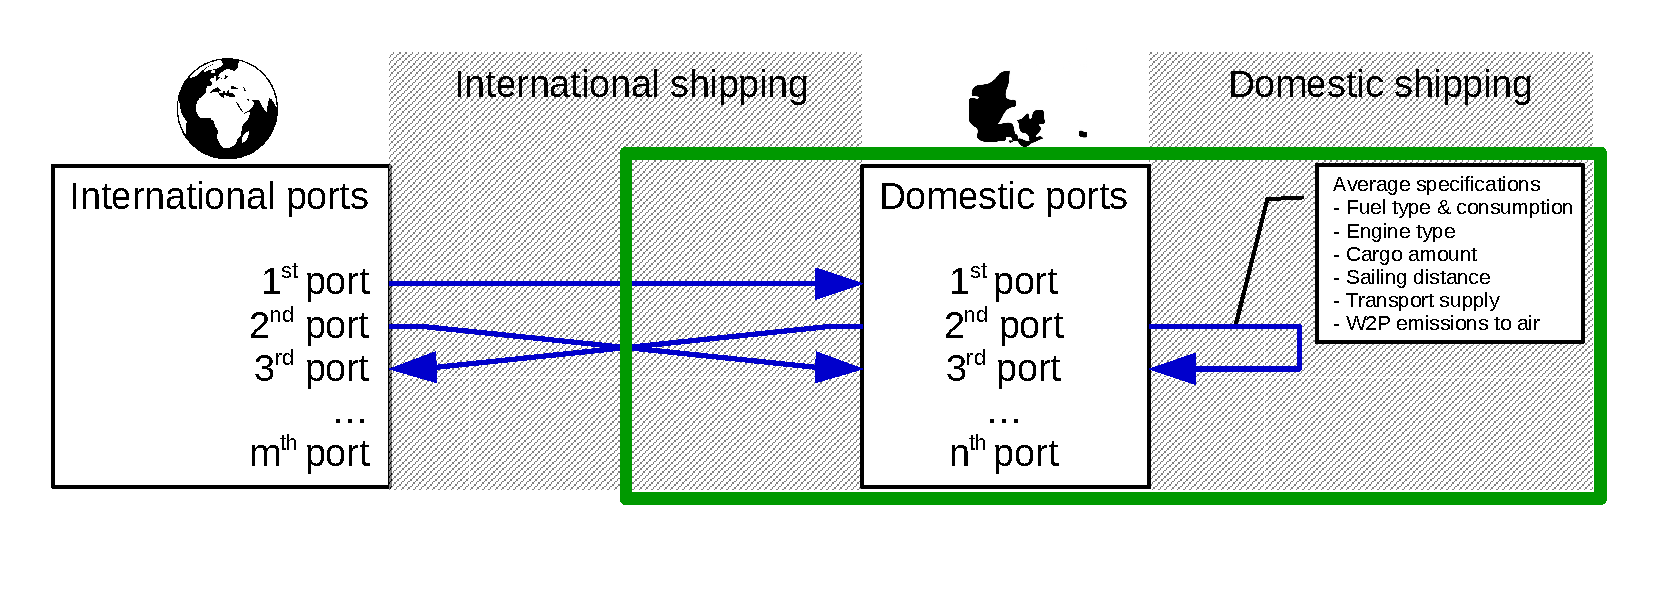
\includegraphics[width=\textwidth]{figures/model_boundary_paper.pdf}
    \caption{Model boundary: The model considers the specifications inside the green box.}
    \label{fig:model_boundary}
\end{figure}

\subsection{Model Structure}
\label{subsec:Structure}
While the core components of the model are the equations describing the objective function of the optimisation as well as constraints, pre-processing of the input and post-processing of the output data constitute an important part of the modelling framework. \cref{fig:model_boxflow} illustrates the model flow with white boxes representing data instances, blue arrows processes. These scripts are written in Python with the pre-processing applying the data package \textit{panda}, the optimisation utilising the optimisation package \textit{pyomo} and the output processing additionally to pandas \textit{mathplotlib} for illustrating the results in plots. All scripts, raw and processed data including documentation are available on github \cite{GitHub2018}, where further development of the model takes place. To allow for reproducibilty of the presented results, \cite{BenBrahim2018} points to the version of data and code deployed for this research. Both are published under the GNU general public license version 3.

\begin{figure}[tbh]
    \centering
    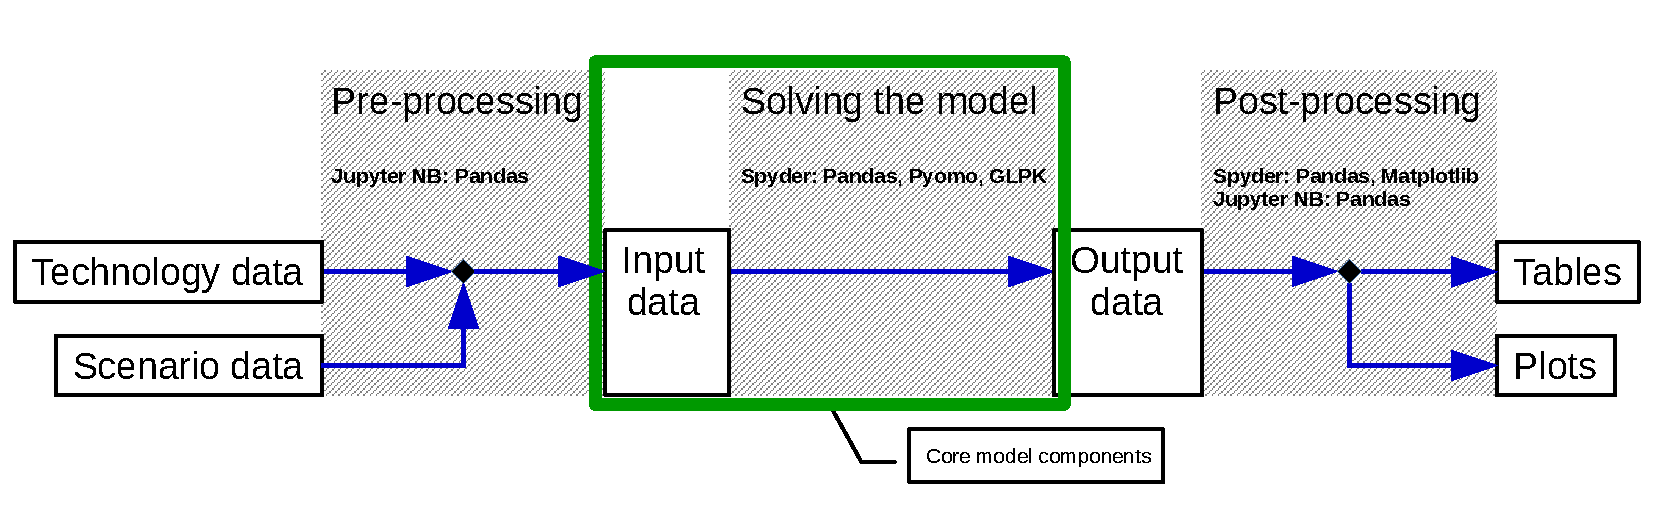
\includegraphics[width=\textwidth]{figures/model_boxflow_paper.pdf}
    \caption{Model boxflow: The core model consists of the components inside the green box.}
    \label{fig:model_boxflow}
\end{figure}

\subsection{Mathematical Formulation}
\label{subsec:Mat}
The problem is formulated in a linear, divisible manner, aiming to minimise the objective function. Model variables in first time step 2016 are initialised with data compiled for the current Danish shipping fleet. Later, constraints trigger the necessary investment decisions for new technologies and scrap existing ships not in compliance with legal obligations or emission targets. Since the objective's sense is the minimisation of the overall total system's costs \cref{eq:objective}, investments are interpreted as adverse, yet inevitable actions to cope with the constraint's demands, such as: Lowering CO$_2$e emissions to air, (over-)supplying the transport demand in each time step or scrapping ships. All model variables domains are within non-negative real numbers, including zero $\left(R_{0}^{+}\right)$. The nomenclature used in the equations and table headers in the following sections is given in the nomenclature list.
\glsdisablehyper
\glsaddall
\begin{table*}[thb]
%\renewcommand\tablename{Nomenclature list}
\begin{mdframed}
\footnotesize{
%\begin{mdframed}[style=mdfexample1]
\begin{multicols}{2}
\printglossary[style=tree,type=a]
\vspace{-0.3cm}
\printglossary[style=tree,type=s]
\vspace{-0.3cm}
\printglossary[style=tree,type=v]
\vspace{-0.3cm}
\printglossary[style=tree,type=p]
\end{multicols}
}
\end{mdframed}\label{box:nomenclature}
\caption*{Nomenclature list.}
\end{table*}

\subsubsection{Model objective}
The objective equation aims at minimising the systems total expenditures over all time steps and ship types. It comprises the sum of each years costs for fuel consumption, additional infrastructure as well as ship capacity. Costs for fixed assets -- fuel infrastructure and ships -- are given as annuities and account only with the annual added capacities. Besides, their existing amount in 2016 ($fainit_{t,s}$ in $T_0$) is not cost-effective and therefore subtracted from $CI$ and $CS$.
\begin{subequations}
    \begin{align}
        min. &\sum_{\forall t \in T}\sum_{\forall s \in S}\left( CF_{t, s} + CI_{t, s} + CS_{t, s} \right)\label{eq:objective}\\
        \intertext{s.t.}
        CF_{t, s} &\geq fa_{t,s} \cdot cf_{t,s}\\
        CI_{t, s} &\geq \left( faiup_{t,s} - fainit_{t, s} \right) \cdot li_{s} \cdot ci_{t,s}, \forall t \in T_0\\
        CI_{t, s} &\geq faiup_{t,s} \cdot li_{s} \cdot ci_{t,s}, \forall t \in T_{>0}\\
        CS_{t, s} &\geq \left( fasup_{t,s} - fainit_{t, s} \right) \cdot ls_{s} \cdot cs_{t,s}, \forall t \in T_0\\
        CS_{t, s} &\geq fasup_{t,s} \cdot ls_{s} \cdot cs_{t,s}, \forall t \in T_{>0}
    \end{align}
\end{subequations}

\subsubsection{Constraints on fuel utilisation}
Fuel constraints may apply for a selection of ship types and years in the model. With regard to infrastructure and ships, only the incremental capacity is cost effective while taking into account expiry dates of existing capacities. The expiry dates relate to the technical lifetimes, which differ among ships and infrastructure, also when of same type.\\\par\noindent
\textit{Infrastructure capacity: }Defined as the sum of all additional fuel infrastructure build during the elapsed technical lifetime.
\begin{subequations}
    \begin{align}
        faicap_{t,s} &\leq \sum_{\textbf{x}}^{t-1} \left( faiup_{x,s} \right), \forall t \in T_{>0}, \forall s \in S\label{eq:faicap}\\
        \intertext{s.t.}
        x &= T_0, \forall t \leq \left(li_{s} + T_0 - 1\right)\\
        x &= t - li_{s} + 1, \forall t > \left(li_{s} + T_0 - 1\right)
    \end{align}
\end{subequations}\\
\textit{Additional infrastructure: }Additional fuel infrastructure in order to supply the fleet.
\begin{equation}
    faiup_{t,s} \geq fa_{t,s} - faicap_{t,s}, \forall t \in T_{>0}, \forall s \in S\label{eq:faiup}
\end{equation}\\
\textit{Ship capacity: }Defined as the sum of all additional shipping capacity build during the elapsed technical lifetime.
\begin{subequations}
    \begin{align}
        fascap_{t,s} &\leq \sum_{\textbf{x}}^{t-1} \left(fasup_{x,s} \right), \forall t \in T_{>0}, \forall s \in S\label{eq:fascap}\\
        \intertext{s.t.}
        x &= T_0, \forall t \leq \left(ls_{s} + T_0 - 1\right)\\
        x &= t - ls_{s} + 1, \forall t > \left(ls_{s} + T_0 - 1\right)
    \end{align}
\end{subequations}\\
\textit{Additional ships: }Additional ships in order to supply the cargo transport required.
\begin{equation}
    fasup_{t,s} \geq fa_{t,s} - fascap_{t,s}, \forall t \in T_{>0}, \forall s \in S\label{eq:fasup}
\end{equation}\\
\textit{Refit capacity: }Defines for each year the old ship's capacity possible to refit.
\begin{subequations}\label{eq:refitships}
    \begin{align}
    fa_{t,s} + fa_{t,r} - fa_{T_0, s} &\leq 0, \forall t \in T_{<\left(T_0+ls_{s}\right)}, \forall s, r \in RO\\
    fa_{t,s} + fa_{t,r} & = 0, \forall t \in T_{\geq\left(T_0+ls_{s}\right)}, \forall s, r \in RO
    \end{align}
\end{subequations}\\
\textit{Bio-fuel capacity: }Defines for each year the upper limit of bio-fuel available.
\begin{equation}
    \sum_{\forall s \in SB} \left(fa_{t,s} \right) - ba_{t} \leq 0, \forall t \in T\label{eq:biofuel}
\end{equation}

\subsubsection{Constraints on transport demand}
Transport demand constraints may apply for a selection of ship types and years in the model, depending on the range category -- either short or long -- and the emission regulations -- in- or outside ECAs.\\\par\noindent
\textit{Total transport demand: }Defines for each year that the transport supply per ships must be greater or equal to the total transport demand.
\begin{equation}
    tdtotal_t \leq \sum_{\forall s \in S} \left( fa_{t,s} \cdot ts_{t,s}\right), \forall t \in T \label{eq:td_total}
\end{equation}
\textit{Short transport demand: }Defines for each year the maximum transport supply of all ships categorised as short range.
\begin{equation}
    tdshort_t \geq \sum_{\forall s \in SR} \left( fa_{t,s} \cdot ts_{t,s}\right), \forall t \in T \label{eq:td_short}
\end{equation}
\textit{Non-SECAs transport demand: }Defines for each year the maximum transport supply of all ships only allowed for operation outside of the ECAs.
\begin{equation}
    tdnoneca_t \geq \sum_{\forall s \in SNE} \left( fa_{t,s} \cdot ts_{t,s}\right), \forall t \in T \label{eq:td_noneca}
\end{equation}

\subsubsection{Constraints on emissions}
Emission constraints may apply for a selection of ship types and years in the model. The constraint set imposes limitations to the extend of which certain fuel types are being deployed by the model, based on the CO2e budget and target as well as the legal restrictions defined by the IMO.
\\\par\noindent
\textit{Emission budget: }Defines the amount of accumulated GHG emissions that cannot be exceeded by all ships.
\begin{subequations}
    \begin{align}
    eb &\geq \sum_{\forall t \in T}\sum_{\forall s \in S}\left(EC_{t,s} + EM_{t,s} \right) \label{eq:co2ebudget}\\
    \intertext{s.t.}
    EC_{t,s} &= fa_{t,s} \cdot ec_{t,s}, \forall t \in T, \forall s \in S\\
    EM_{t,s} &= fa_{t,s} \cdot em_{t,s}, \forall t \in T, \forall s \in S
    \end{align}
\end{subequations}\\
\textit{Emission target: }Defines the amount of GHG emissions as of the target year that cannot be exceeded by all ships.
\begin{equation}
    \frac{\sum_{\forall s \in S} \left(EC_{T_0,s}+EM_{T_0,s}\right)}{\sum_{\forall s \in S} \left(EC_{t,s}+EM_{t,s}\right)} \cdot et \geq 1, \forall t \in T_{\geq \left(etyr-T_0\right)}
\end{equation}\\
\textit{Global SO$_X$ regulations: }Defines the set of ships as of 2020 prohibited to operate globally with respect to global SO$_X$ regulations.
\begin{equation}
    fa_{t,s} = 0, \forall t \in T_{\geq slnonecayr-T_0}, \forall s \in SNG \label{eq:sox_global}
\end{equation}\\
\textit{NO$_X$ regulations: }Defines the set of ships as of 2021 prohibited to operate within NECAs.
\begin{equation}
   fa_{t,s} = 0, \forall t \in T_{\geq tlecayr-T_0},\forall s \in NT \label{eq:tier}
\end{equation}


\subsection{Data}
\label{subsec:Dat}
The fuel and ship data tables contain both, information about the status-quo of the Danish maritime industry and future investment options for alternative means of shipping. For fuel data, the unique identifier is the fuel type, for ship data it is ship type. Ship types can use the same fuel type but different engine types (IC, FC, EM).

\subsubsection{Fuel data}
The fuel parameters (\cref{tab:fuel_data}) include CO$_2$ and CH$_4$ emission factors (well-to-tank), sulphur content as well as cost parameters. The latter include fuel as well as infrastructure costs and its respective lifetime. For the fuels currently applied on a large scale (HFO, MDO, BDO), the bunker index prices are taken. It is assumed that these include all cost components from well to tank including fixed costs for a sufficient supply infrastructure. Thus, for these, infrastructure and fuel costs are not further specified. In contrast, new fuel technology costs are divided into fixed and variable components, since sufficient supply infrastructure has not been installed. For the necessary cases, fuel upgrading is assumed to be done at berth to elude additional grid investments. as the gas grid could handle any conceivable amount of natural or upgraded bio-gas transport.
\begin{table}[htb]
    \centering
    \resizebox{\textwidth}{!}{
    \begin{tabular}{lrrrrrrrr}
        \toprule
        Fuel type & cf & ci & cf + ci & ec(w2t) & em(w2t) & sulphur content & li & References \\
        & $\left[\frac{EUR_{2016}}{GJ_{fuel}}\right]$ & $\left[\frac{EUR_{2016}}{GJ_{fuel}}\right]$ & $\left[\frac{EUR_{2016}}{GJ_{fuel}}\right]$ & $\left[\frac{g_{co2}}{MJ_{fuel}}\right]$ & $\left[\frac{g_{ch4}}{MJ_{fuel}}\right]$ & $\left[\%_{mass}\right]$ & $\left[a\right]$ & \\
        \midrule
        HFO   & -        & -        & 6.547     & 8.148         & 0.090            & 2.9525   & 40   & \cite{BIX2018,Gilbert2018,Bengtsson2012,BRYNOLF2014}    \\
        MDO   & -        & -        & 12.775    & 7.728         & 0.090            & 0.7500   & 40   & \cite{BIX2018,Gilbert2018,Bengtsson2012,Andersson2015}    \\
        BDO   & -        & -        & 24.240    & 0             & 0.030            & 0.1498   & 40   & \cite{SSI2018,Bengtsson2012}    \\
        LNG   & 4.888    & 0.139    & -         & 6.600         & 0.033            & 0.0500   & 36   & \cite{EnerginNet2018,Gilbert2018,BRYNOLF2014,Andersson2015}    \\
        LBG   & 27.847   & 1.599    & -         & 0             & 0.130            & 0.0750   & 25   & \cite{Brynolf2018,Bengtsson2012}    \\
        H2    & 20.885   & 1.199    & -         & 0             & 0                & 0        & 25   & \cite{Brynolf2018}    \\
        CH3OH & 29.240   & 1.679    & -         & 0             & 0.042            & 0.0912   & 25   & \cite{Brynolf2018,BRYNOLF2014}    \\
        NH3   & 26.803   & 1.802    & -         & 0             & 0                & 0        & 20   & \cite{Morgan2017}    \\
        ELEC  & 13.889   & 2.929    & -         & 0             & 0                & 0        & 20   & \cite{Vree2008}    \\
        \bottomrule
    \end{tabular}}
    \caption[Fuel type data]{Fuel type data for each parameter (for abbreviations see the nomenclature list in \cref{box:nomenclature}).}
    \label{tab:fuel_data}
\end{table}

\subsubsection{Ship and technology data}
Ship-type input parameter (see \cref{tab:ship_data}) include emission factors, compliance with sulphur and NO$_x$, lifetime, options for refit, costs, transport supply as well as application options regarding range. Additionally, the amounts of fuels used today are applied as the starting point. For the future, the amount is determined endogenously by the model.

The emission factors for CO$_2$ and CH$_4$ only include the tank-to-propeller emissions, since the upstream emissions are already covered by the fuel data. Regarding sulphur and NO$_x$ compliance, Tier rating defines if a ship complies with IMO NO$_x$ regulations and can thus be driven in a NECA. Old ships in the model do not have sufficient TIER rating and thus either have to be scrapped or refitted when the regulation entries into force in 2021. New built ships are generally assumed to have a TIER 3 rating. Scrubber installations are defined for each ship type.

The average remaining lifetime for existing ships is 11 years since the average age of the current fleet is 14 years, when considering bulk, container and tanker ship types that dominate the Danish cargo fleet \cite[Tab.~2.2, p.~27]{UNCTAD2017}. Refitting an old ship to comply with new regulation can possibly be an option to reduce costs. A typical refit currently ongoing to comply with sulphur regulations is the installation of a scrubber for ships with internal combustion engines running on HFO. It has to be mentioned that this results in a reduction of specific transport per fuel due to efficiency losses caused by the scrubber. Ships with internal combustion engine using HFO can also be refitted for the use of BDO, which is relatively straightforward and thus does not imply much costs. These kind of refits do not extent the lifetime of the ship or technology, but just provide different functionality.

Regarding the range options, only full electric ships are restricted to radius of 500 nautical miles (926 km), all other have an unlimited range.

\begin{table}[htb]
    \centering
    \resizebox{\textwidth}{!}{
    \begin{tabular}{llrrrrrrrrrrr}
        \toprule
                       Ship-type & Range & ls & fa$_{2016}$ & ts & cs & ec(t2p) & em(t2p) & Refit & Refit opt. & Tier & Scrubber & References \\
                       &       & $\left[a\right]$ & $\left[PJ_{fuel}\right]$ & $\left[\frac{Ttkm}{GJ_{fuel}}\right]$ & $\left[\frac{EUR_{2016}}{GJ_{fuel}}\right]$ & $\left[\frac{g_{CO2}}{MJ_{fuel}}\right]$ & $\left[\frac{g_{CH4}}{MJ_{fuel}}\right]$ & & & & & \\
        \midrule
        IC HFO (old)   & long  & 11     & 9.93   & 9.69        & 8.72     & 76.06            & 0.00045          & yes   & IC HFO (refit) & 0           & no     & \cite{UNCTAD2017,Eurostat2018,Wisdom2017,Kristensen2012,Rex2017} \\
        IC MDO (old)   & long  & 11     & 5.99   & 9.40        & 8.45     & 74.36            & 0.00045          & yes   & IC BDO (refit) & 0           & yes    & \cite{UNCTAD2017,Eurostat2018,Wisdom2017,Kristensen2012,Rex2017} \\
        IC HFO         & long  & 25     & 0      & 9.40        & 8.45     & 75.90            & 0.00045          & no    &                & 3           & yes    & \cite{UNCTAD2017,Kristensen2012,Rex2017} \\
        IC MDO         & long  & 25     & 0      & 9.40        & 8.45     & 74.32            & 0.00045          & no    &                & 3           & yes    & \cite{UNCTAD2017,Kristensen2012,Rex2017} \\
        IC HFO (refit) & long  & 11     & 0      & 9.40        & 0.02     & 75.90            & 0.00045          & no    &                & 3           & yes    & \cite{UNCTAD2017,McGill2013} \\
        IC BDO (refit) & long  & 11     & 0      & 9.40        & 0        & 0                & 0.00045          & no    &                & 3           & yes    & \cite{UNCTAD2017,Wisdom2017} \\
        IC BDO         & long  & 25     & 0      & 9.40        & 8.45     & 0                & 0.00045          & no    &                & 3           & yes    & \cite{UNCTAD2017,Bengtsson2012} \\
        IC LNG         & long  & 25     & 0      & 10.13       & 96.98    & 54.36            & 0.71000          & no    &                & 3           & no     & \cite{UNCTAD2017,Kristensen2012,Rex2017} \\
        IC LBG         & long  & 25     & 0      & 10.13       & 96.98    & 0                & 0.79000          & no    &                & 3           & no     & \cite{UNCTAD2017,Bengtsson2012} \\
        IC H2          & long  & 25     & 0      & 10.13       & 109.29   & 0                & 0                & no    &                & 3           & no     & \cite{UNCTAD2017,ElGohary2013} \\
        IC CH3OH       & long  & 25     & 0      & 10.13       & 109.29   & 0                & 0.79000          & no    &                & 3           & no     & \cite{UNCTAD2017,Andersson2015,BRYNOLF2014} \\
        IC NH3         & long  & 25     & 0      & 10.13       & 109.29   & 0                & 0                & no    &                & 3           & no     & \cite{UNCTAD2017} \\
        FC LNG         & long  & 25     & 0      & 22.47       & 134.80   & 54.36            & 0.22763          & no    &                & 3           & no     & \cite{UNCTAD2017,VanBiert2016} \\
        FC LBG         & long  & 25     & 0      & 22.47       & 134.80   & 0                & 0.22763          & no    &                & 3           & no     & \cite{UNCTAD2017,VanBiert2016} \\
        FC H2          & long  & 25     & 0      & 22.47       & 134.80   & 0                & 0                & no    &                & 3           & no     & \cite{UNCTAD2017,USDE2015} \\
        FC CH3OH       & long  & 25     & 0      & 22.47       & 134.80   & 0                & 0.22763          & no    &                & 3           & no     & \cite{UNCTAD2017,VanBiert2016} \\
        FC NH3         & long  & 25     & 0      & 22.47       & 134.80   & 0                & 0                & no    &                & 3           & no     & \cite{UNCTAD2017} \\
        EM ELEC        & short & 30     & 0      & 11.86       & 1,047.05 & 0                & 0                & no    &                & 3           & no     & \cite{DNVGL2015} \\
        WIND ELEC      & long  & 30     & 0      & 35.58       & 2,094.11 & 0                & 0                & no    &                & 3           & no     &  \\  
    \bottomrule
    \end{tabular}}
    \caption[Ship type data]{Ship type data for each specific parameter (for abbreviations see the nomenclature list in \cref{box:nomenclature}).}
    \label{tab:ship_data}
\end{table}

\subsubsection{Emission budget}
\label{subsec:em_budget}
The remaining emission budget of CO$_2$e for the temporal scope of the model is a decisive constraint in the calculation. Since there are no agreed or standardised ways of attributing GHG emissions from international shipping to countries, we devised a method that distributes global shipping emissions to countries while keeping as a sum the global carbon budget. We apply a global emission budget estimate by the IPCC \cite[Tab.~SPM.3, RCP2.6]{IPCC2013}. The budget share assigned to shipping is derived from ICCT \cite{Olmer2017}.

Comparison of global maritime CO$_2$e emissions in 2012 with the Danish emissions in 2016 and its application to the global maritime budget leads to the Danish GHG budget. The absolute level of Danish cargo shipping emissions of 1.2 Mt CO2e in 2016 is derived from the fuel specific emission operation factors, multiplied by total fuel consumed in that year. The relation of global maritime emissions in 2012 with the Danish in 2016 leads to rather over-estimated Danish budget since the global transport demand was increasing in that period \cite[Tab.~1.3,~p.~5]{UNCTAD2017}. Keeping the resulting emission level constant would deplete the budgets within the next 15 years and allows for less GHG emissions compared to a linear decrease from today until 2050.
\begin{table}[htb]
    \centering
    \begin{tabular}{llrr}
        \toprule
         & Unit & CO2e emissions & References \\
         \midrule
         Global budget & $\left[Mt\right]$ & 510000 & \cite{IPCC2013} \\
         Global maritime budget share & $\left[\%\right]$ & 3 & \cite{Olmer2017} \\
         Global maritime budget & $\left[MT\right]$ & 15300 &\\[1.5ex]
         Global maritime emissions in 2012 & $\left[Mt\right]$ & 961 & \cite{Smith2014} \\
         Danish maritime emissions in 2016 & $\left[Mt\right]$ & 1.2 & \cite{Kristensen2012,Eurostat2018,Wisdom2017} \\
         Danish maritime emission share & $\left[\%\right]$ & 0.125 &\\[1.5ex]
         Danish budget & $\left[Mt\right]$ & \textbf{19.12} & \\
         \bottomrule
    \end{tabular}
    \caption{Derivation of CO$_2$e emission budget from global to Danish level.}
    \label{tab:dk_em_budget}
\end{table}


\subsection{Scenarios}
\label{subsec:Sce}
In general, all scenarios are manipulations of the reference scenario's input parameters, where one or a cluster of parameters are changed in a ceteris paribus manner and by the same percentage. If appropriate, changing rates are clustered, due to market coupling effects, I.e. electro-fuels, as they all depend primary on electricity.

\subsubsection{Scenario data}
The development of cost and other parameters is decisive for the model results. To make the assumptions behind that transparent, the variations are expressed as percentage change rates from 2016 to 2050 (\cref{tab:ref_rates}). Derived from that number, annual changing rates are applied, thus, the respective parameter change over the whole time span of the model is exponential, not linear.

\cref{tab:ref_rates} shows the parameter changes and thus future development of the reference scenario.

Other decisive parameters are bio-fuel availability and transport demand. Bio-fuel availability increases from 0 \% in 2016 to 40 \% in 2050 in relation to the total fuel consumption in 2016 (\cite{DEA2016}). The transport demand stays constant based on \cite[p.~18]{ITF2018} and \cite[p.~19]{Rex2017}.

\begin{table}[htb]
    \centering
    \resizebox{\textwidth}{!}{%
    \begin{tabular}{lrcr}
        \toprule
        Modified & Percentage change & Affected Technologies & References \\
        parameters & from 2016 to 2050 & & \\
        \midrule
        ic  & -20   & LNG,LBG,H2,CH3OH,NH3,ELEC         & \cite[fig.~6,~p.~13]{Brynolf2018}     \\
        cf  & 110   & HFO,MDO,BDO,LNG                   & \cite[fig.~13,~p.~3]{JAE-KNY/MDA2017} \\
            & -20   & LBG,H2,CH3OH,NH3,ELEC             & \cite[fig.~6,~p.~13]{Brynolf2018}     \\
        cs  & -40   & IC: LNG,LBG,H2,CH3OH,NH3          & \cite{Rex2017}                        \\
            & -50   & FC: LNG,LBG,H2,CH3OH,NH3          & \cite{Rex2017}                        \\
            & -75   & EM,WIND: ELEC                     & \cite{Rex2017}                        \\
        ts  & +15   & All except old ships              & \cite[tab.~51,~p.~282]{Smith2014}     \\
        ec  & -10   & IC: HFO,MDO,LNG; FC: LNG          & \cite[tab.~51,~p.~282]{Smith2014}     \\
        em  & -10   & IC: HFO,MDO,BDO,LNG; FC: LNG,LBG  & \cite[tab.~51,~p.~282]{Smith2014}     \\
        \bottomrule
    \end{tabular}}
    \caption{Change of fuel and ship specific parameters from 2016 to 2050 in the Reference scenario (for abbreviations see the nomenclature list in \cref{box:nomenclature}).}
    \label{tab:ref_rates}
\end{table}

\subsubsection{Scenario overview}
\cref{tab:scn_overview} gives a scenario overview with abbreviation description and manipulated parameters per scenario. In total 15 scenarios where conducted. The extent to which the respective scenario parameters are modified is stated alongside the results in \cref{sec:Results}.

\begin{table}[thb]
    \centering
    \resizebox{\textwidth}{!}{%
    \begin{tabular}{lll}
        \toprule
        Scenario & Description & Modified \\
        & & parameters \\
        \midrule
        REF     & Reference scenario, based on literature & - \\
        REF(mp) & Reference scenario  + methane leakage phaseout & em \\
        BAU     & Business as usual & eb, et \\
        IMO     & International Maritime Organization & eb, et\\
        TDV     & Transport demand variation & tdtotal \\
        BATW    & Cost variation of battery and wind & cf, ci, cs \\
        BDO     & Cost variation of bio-diesel oil & cf \\
        CH3OH   & Cost variation of methanol & cf, ci, cs\\
        H2      & Cost variation of hydrogen & cf, ci, cs \\
        LBG     & Cost variation of liquefied bio-methane & cf, ci, cs \\
        LBG(mp) & Cost variation of liquefied bio-methane + methane leakage phaseout & cf, ci, cs, em \\
        LNG     & Cost variation of natural gas & cf, ci, cs \\
        LNG(mp) & Cost variation of natural gas + methane leakage phaseout & cf, ci, cs, em \\
        NH3     & Cost variation of ammonia & cf, ci, cs \\
        \bottomrule
    \end{tabular}}
    \caption[Scenario overview]{Scenario overview with description and modified parameters.}
    \label{tab:scn_overview}
\end{table}

\section{Results and Discussion}
\label{sec:Results}
% 2000 words

% BAU compared to IMO, compared to REF

\autoref{fig:BAU} displays the fuel consumption and cumulative CO$_2$-equivalent emissions in the business as usual scenario (BAU) when no GHG regime is in place. Although SO$_X$- and NO$_X$-restriction area applied, no major change in fuel usage can be detected. If no carbon budget is applied, scrubbers instead of fuel switch are the most cost-efficient solution. Applying the IMO goal to halve climate emissions of shipping in 2050 of the IMO does not lead to significant changes except a minor switch to biodiesel instead of heavy fuel oil (see \autoref{fig:IMO}). In comparison, the climate emission budget restriction in the reference scenario  results in a significant fuel switch: Mainly hydrogen in fuel cells and biodiesel with scrubber in internal combustion engines are chosen (see \autoref{fig:REF}). The comparison shows, that without any kind of climate emission restriction, the total cumulative emissions are twice as high and the IMO plans do not have a significant impact. 

\begin{figure}
    \centering
    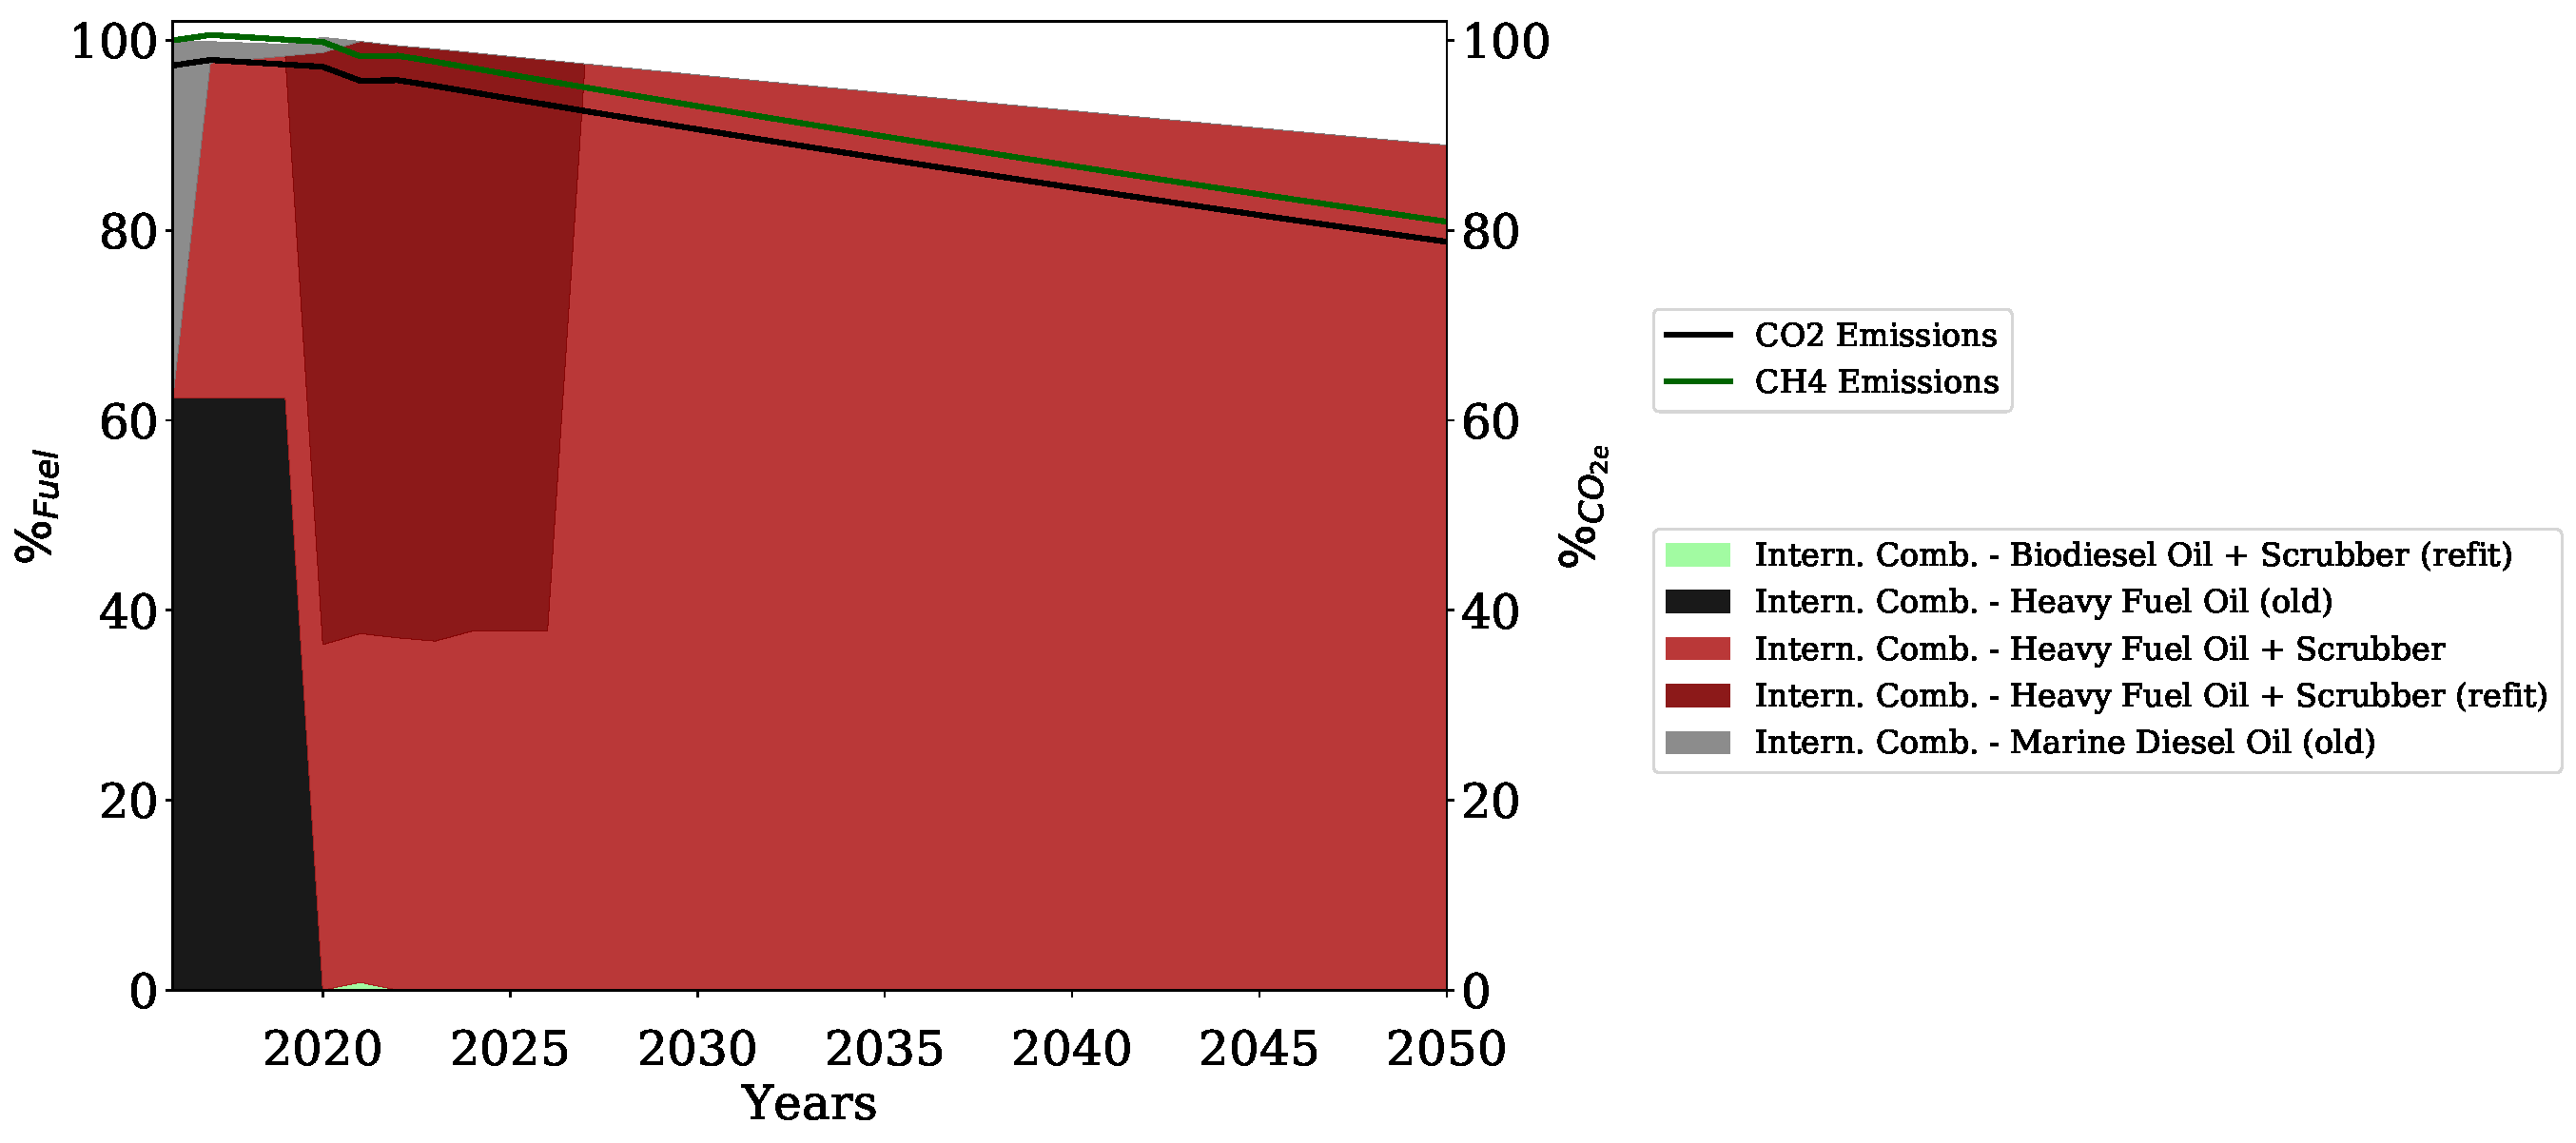
\includegraphics[width=\textwidth]{figures/BAU_fuels_emissions.pdf}
    \caption{Fuel consumption (y-axis left) and cumulative emissions (y-axis right) in the Business-as-usual scenario without carbon budget}
    \label{fig:BAU}.
\end{figure}

\begin{figure}
    \centering
    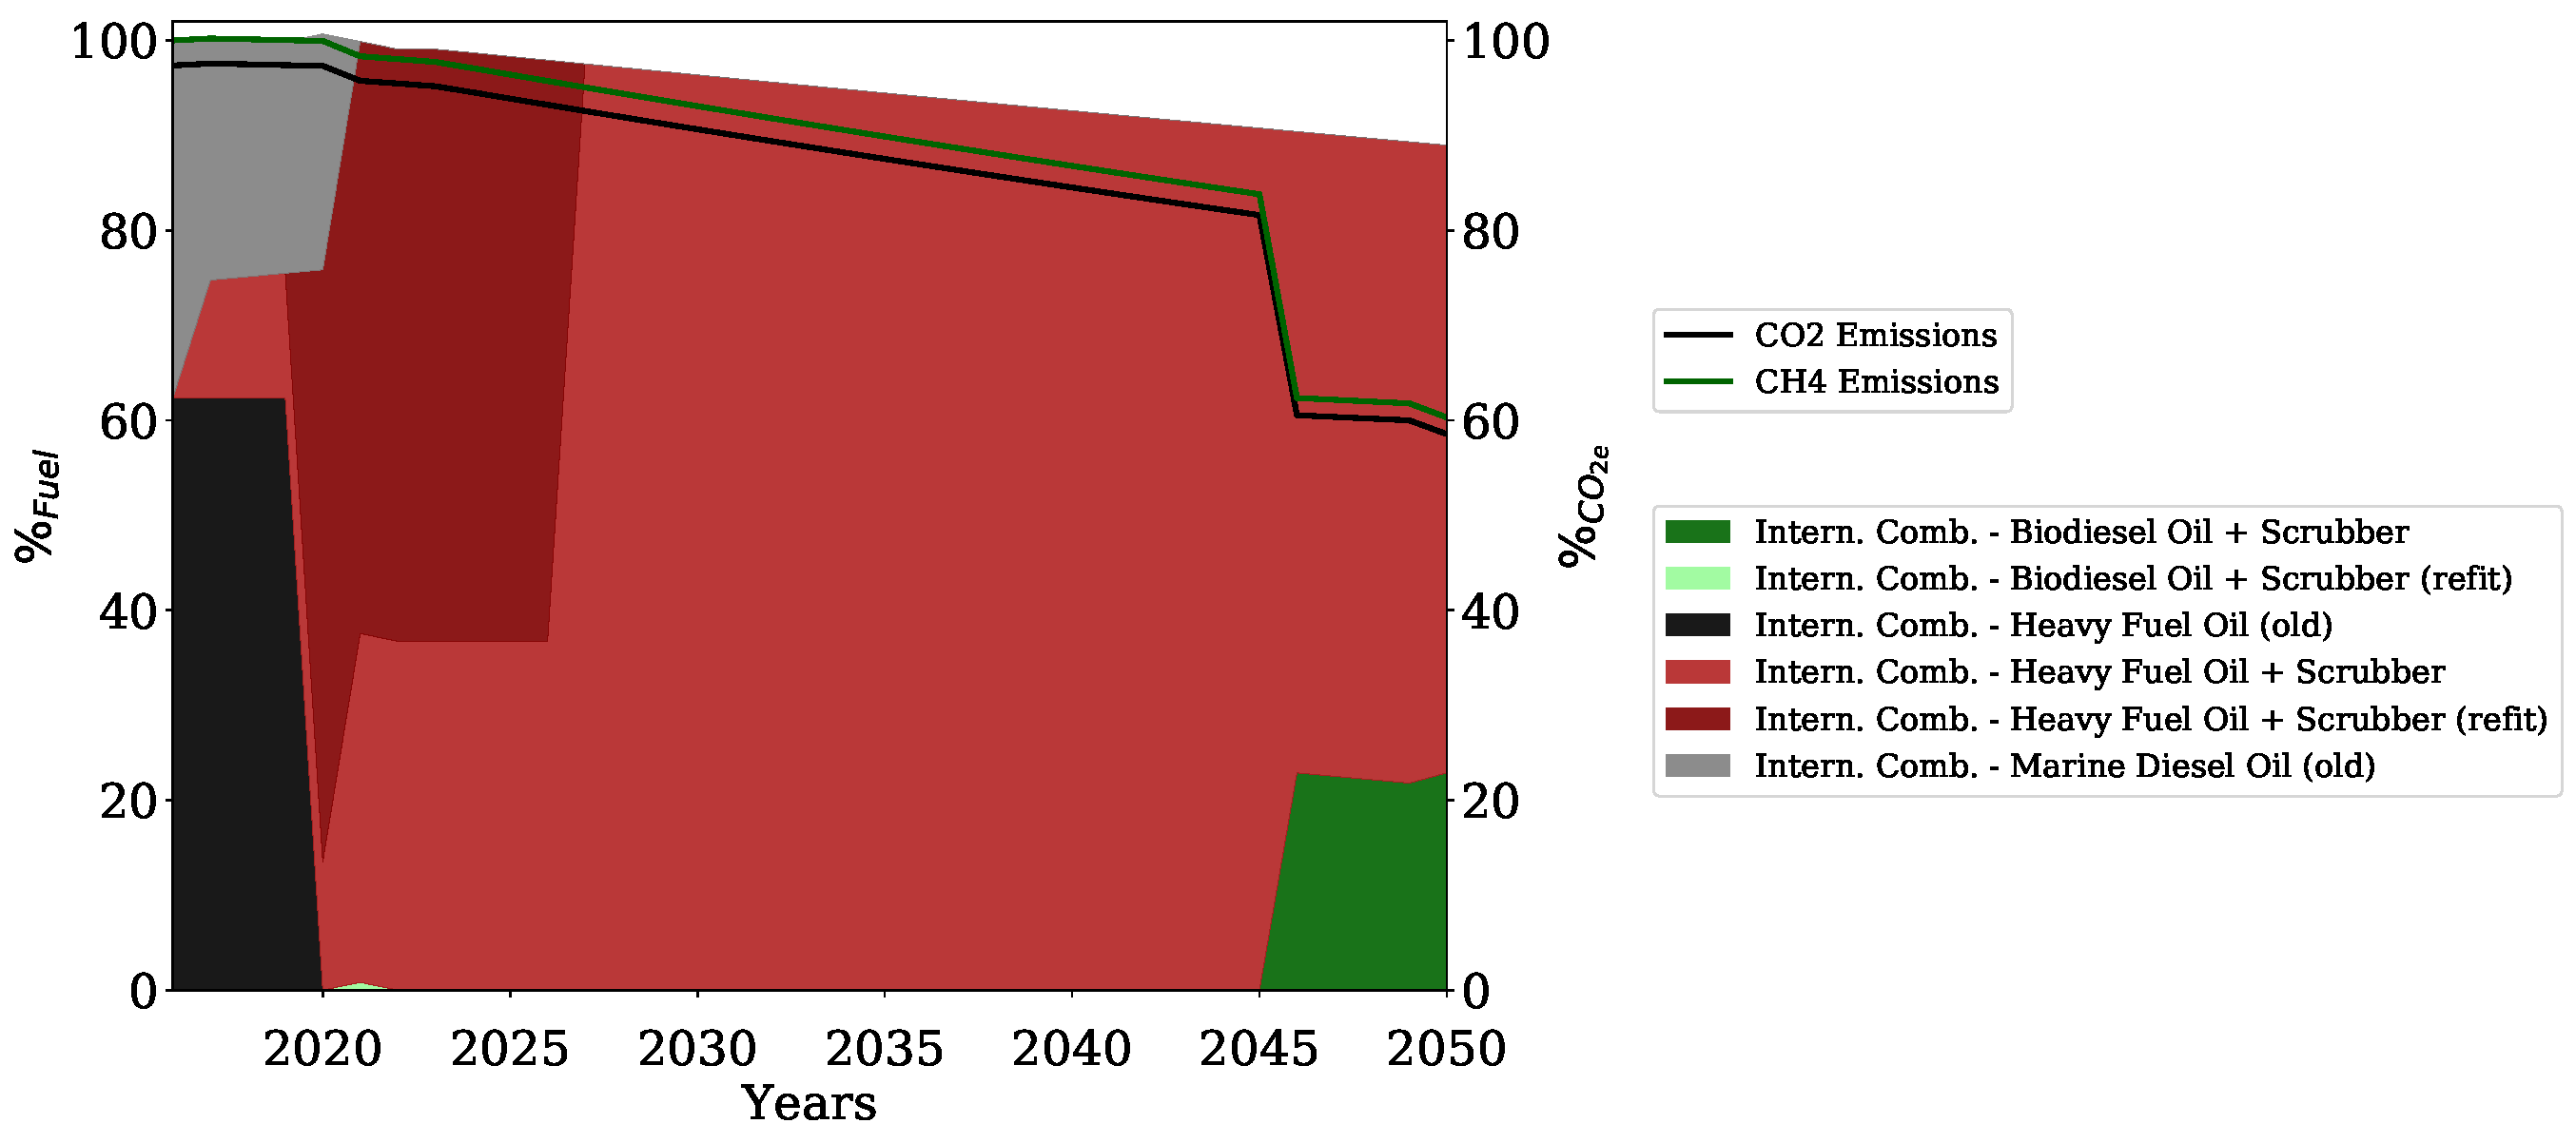
\includegraphics[width=\textwidth]{figures/IMO_fuels_emissions.pdf}
    \caption{Fuel consumption (y-axis left) and cumulative emissions (y-axis right) in the IMO scenario, applying the climate emission target of the International Maritime Organsiation for 2050}
    \label{fig:IMO}
\end{figure}

\begin{figure}
    \centering
    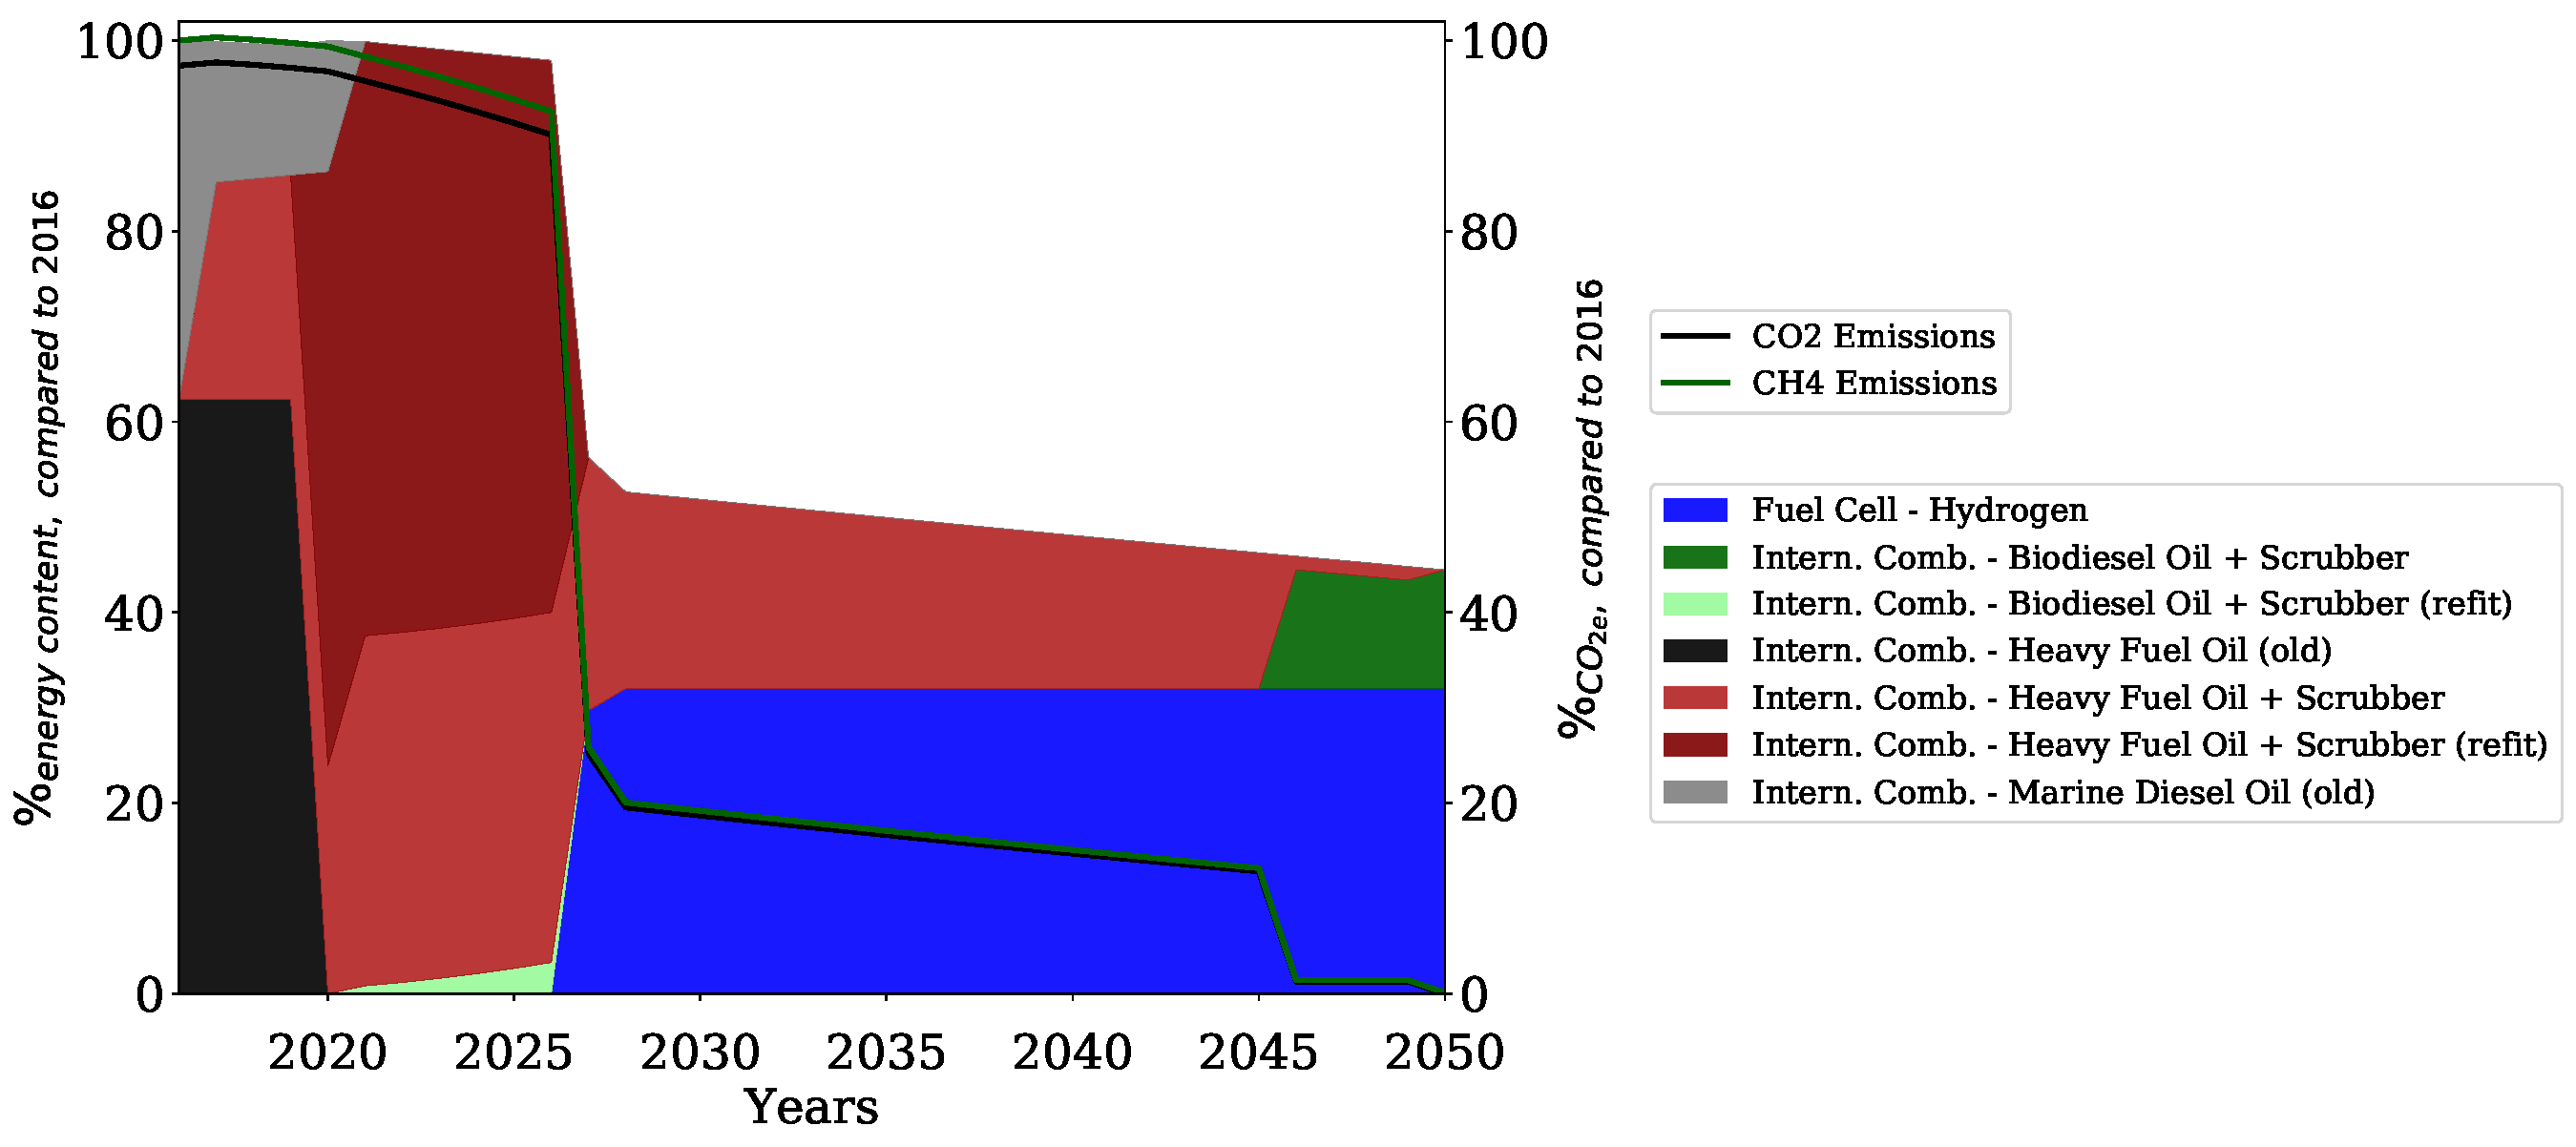
\includegraphics[width=\textwidth]{figures/RS_fuels_emissions.pdf}
    \caption{Fuel consumption (y-axis left) and cumulative emissions (y-axis right) in the Reference scenario with a limited carbon budget}
    \label{fig:REF}
\end{figure}

% REF compared to REF methane leakage?
The comparison between the REF scenario with a methane leakage phase out scenario (see \autoref{fig:RS_MP} illustrates the impact, methane emissions have on the possible application of LNG and LBG in a climate emission reduction regime.

\begin{figure}
    \centering
    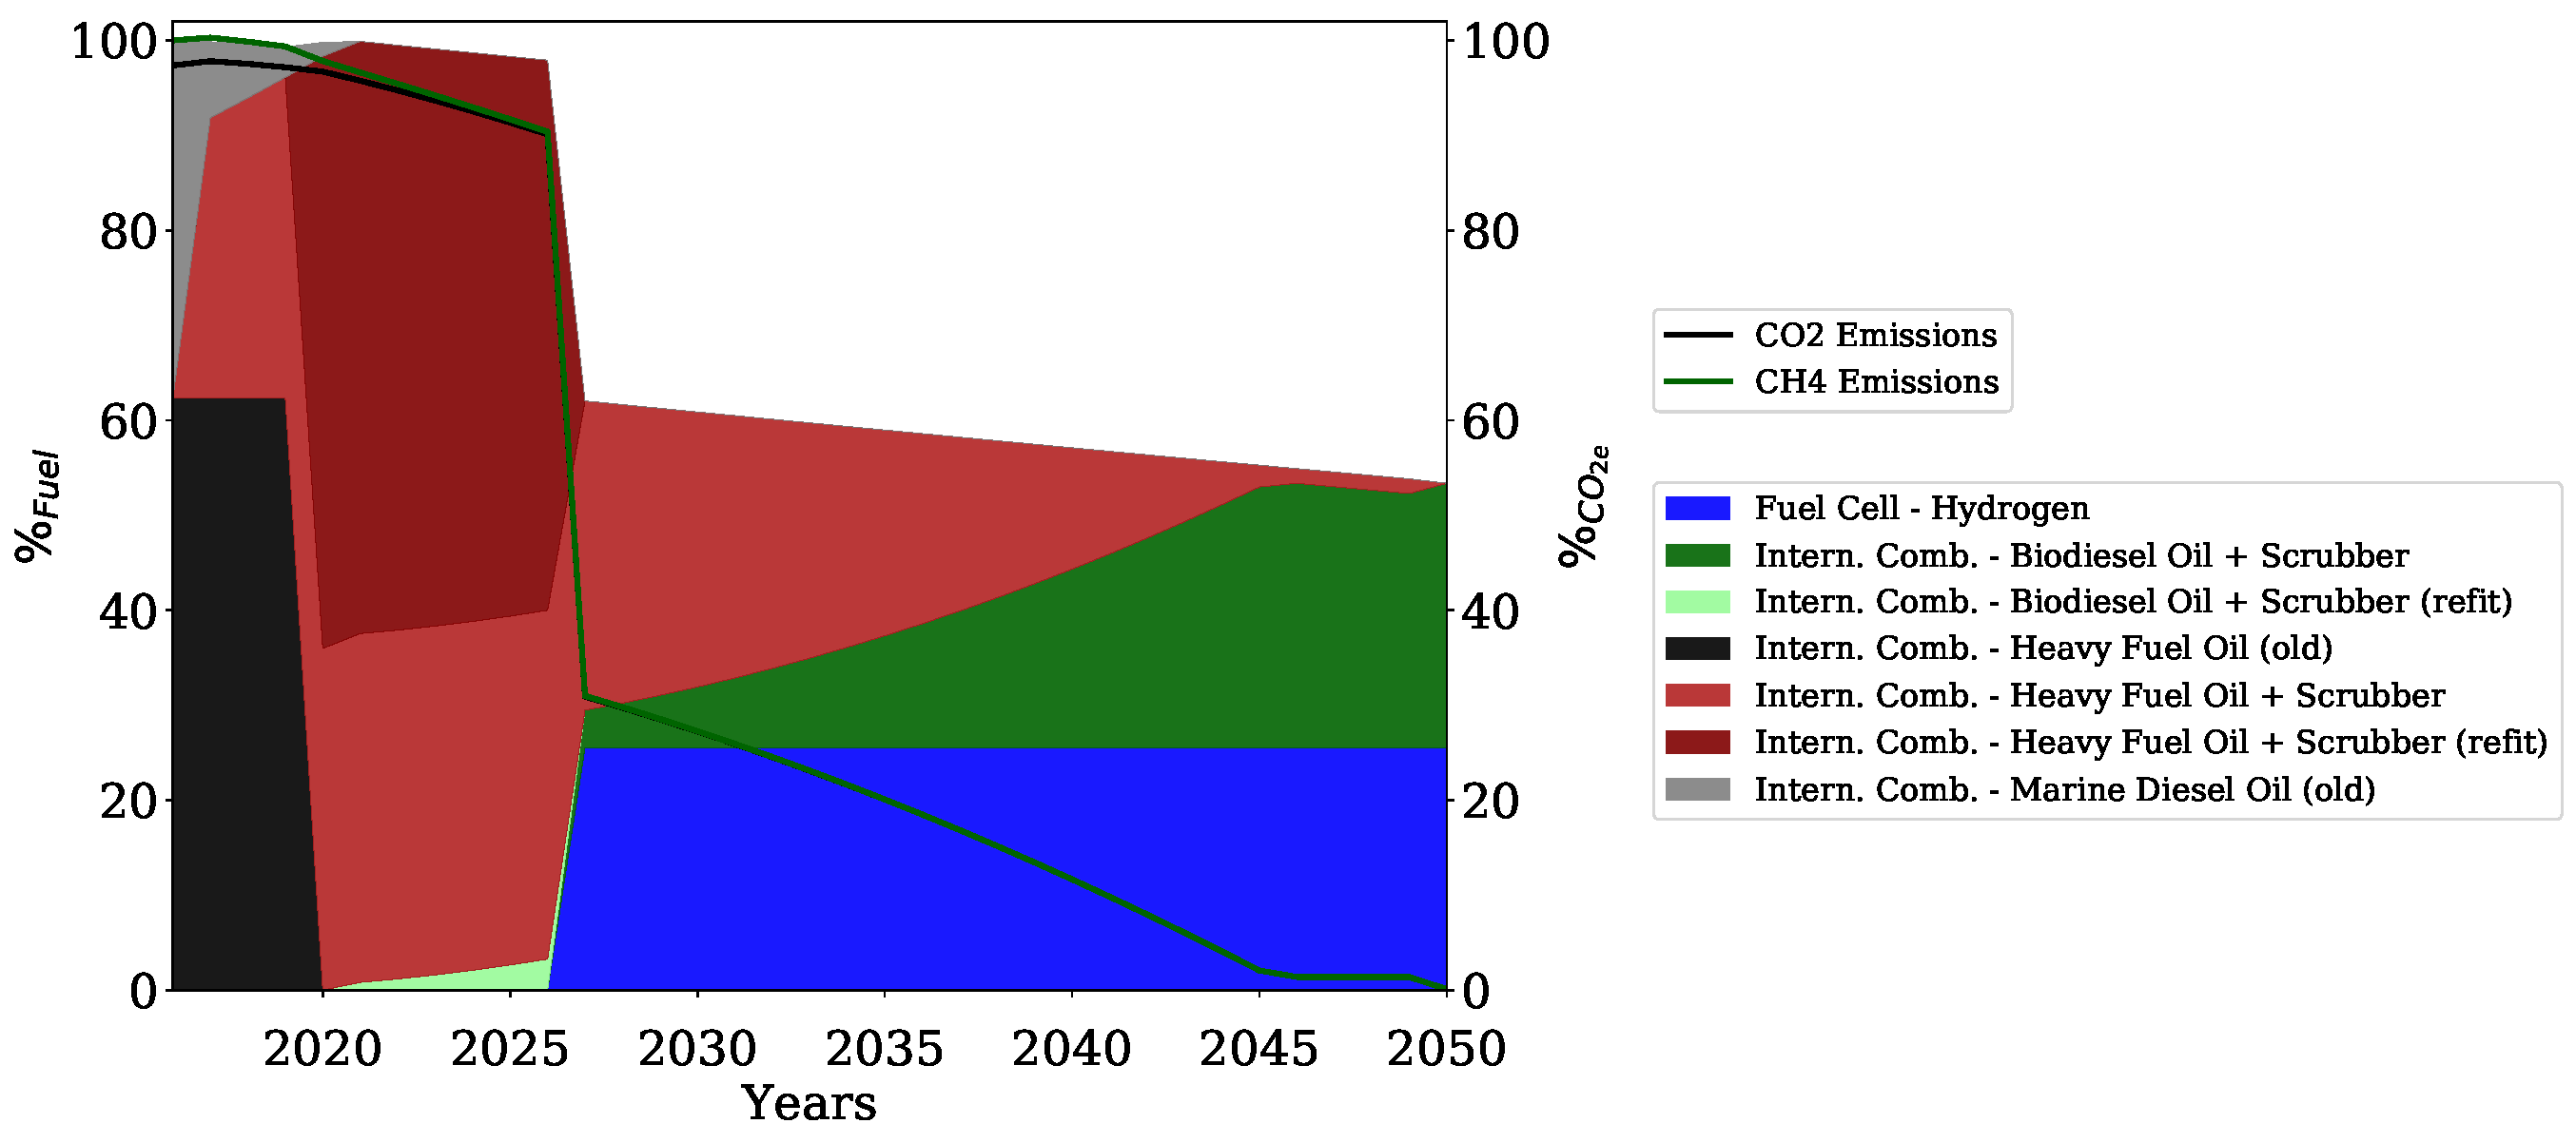
\includegraphics[width=\textwidth]{figures/RS_MP_fuels_emissions.pdf}
    \caption{Fuel consumption (y-axis left) and cumulative emissions (y-axis right) assuming methane leakage phase-out}
    \label{fig:RS_MP}
\end{figure}

% Demand variation - Cheapest?, Cost reduction bigger than transport reduction
% aus Tills Arbeit: Since transport demand declines over time, less investments are needed so that the system costs fall by 25 % to 15 billion EUR2016. These overall cost reductions are much greater than the entire transport demand reduction of 17 %. The faster the demand curves in Fig. 8.12 fall before it reaches the year of major investments into new fuel technologies, the greater this cost benefit would be.


% Cost variation: Methanol and Ammonia are close
Due to the high level of uncertainty of cost development of infrastructure, fuel and propulsion technology of different marine fuel options, a wide range of cost variations is applied to test for its effect on fuel composition. The results are summarised in \autoref{fig:costVariation}. Depending on the cost rate change of a specific fuel technology (x-axis), while keeping all other parameters constant, its share in the total fuel consumption from 2016-2050 (y-axis) changes significantly. The black dashed line at a cost rate change of zero represents the reference scenario. Already at a 10\% cost change rate (including fuel, technology and infrastructure costs), methanol and ammonia respectively gain relevance, reaching a dominant role at a 20\% cost change rate. Thus if the costs of either methanol or ammonia drop by 20\%, these would take over the role of hydrogen as the main renewable fuel of the future.

% LNG is no option, LBG just if methane leakage phase out
For LBG, the development of the methane leakage problem is of outstanding importance. Under the assumption that methane leakage can be coped with until 2050 (dashed line), LBG is close to hydrogen, methanol and ammonia as choice to be the dominate fuel in 2050. Contrary to that, LNG would not only require a methane leakage phase out, but also a very favourable cost development to play a major role.

% BATW has to be decreased significantly, but the conditions applied were rather unfavorable for BATW.
Sailing cargo ships, driven by a combination of wind and electricity from batteries seem to only be cost efficient in case of very strong drops in costs. However, the influence factors have more dimensions than just the pure battery and ship costs. In this model, it is assumed that one third of the propulsion is done by electricity. For long distance cargo, that mainly has to use the engine for manoeuvring into and out of the harbour, the wind share and potentially additional solar input can be significantly increased and thus the required battery and electricity costs reduced.

\begin{figure}[t]
    \centering
    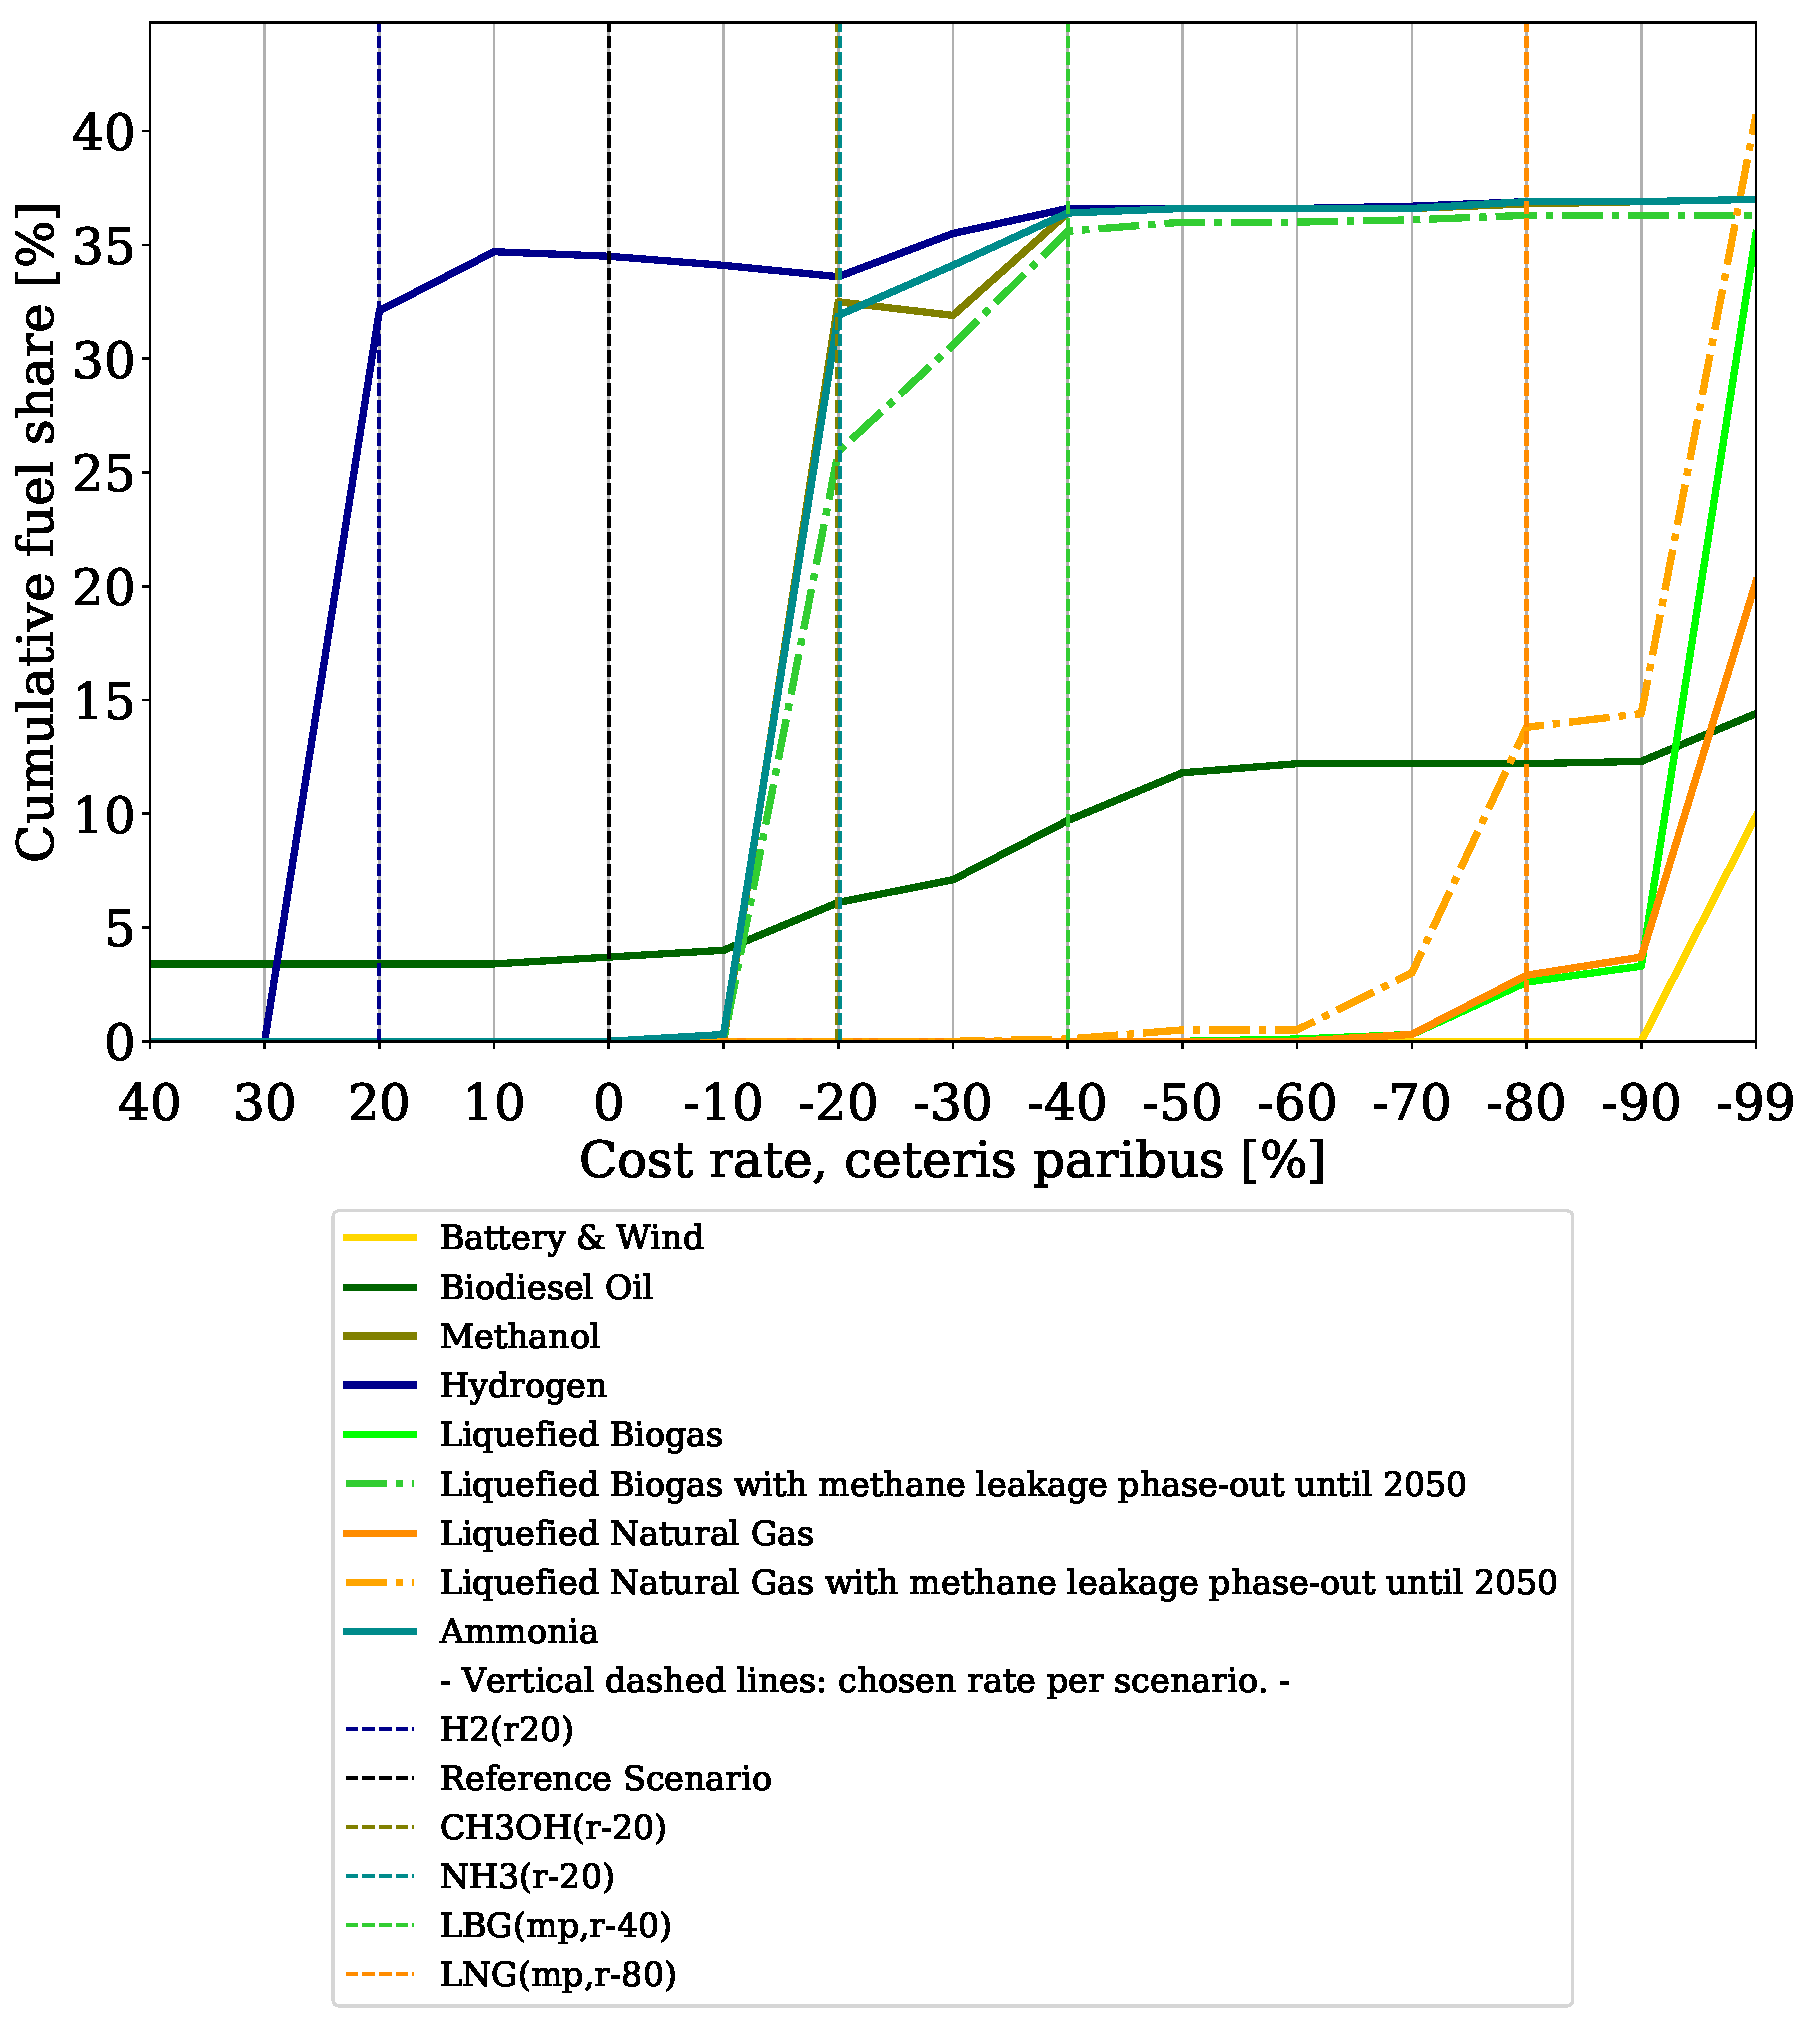
\includegraphics[width=.75\textwidth]{figures/costVariation.pdf}
    \caption{Total fuel shares from 2016-2050 (y-axis) in relation to different cost range changes (x-axis) compared to the reference case}
    \label{fig:costVariation}
\end{figure}

% Compare all scenarios: Fuel composition total and 2050
For comparison, the total fuel use of all scenarios for 2016-2050 is displayed in \autoref{fig:AllFuelTotal} and the fuel composition in the target year 2050 in \autoref{fig:AllFuel2050}. A general efficiency increase can be seen for all carbon budget scenarios. Due to higher operational tank-to-propeller efficiency and thus a higher Tkm/GJfuel - rate, less fuel is applied in the carbon budget scenarios. Except the transport demand scenario all supply the same transport demand.

\noindent
\begin{minipage}[t]{0.49\textwidth}
    \centering
    \captionsetup{justification=centering}
    \captionof{figure}{Total fuel use from 2016-2050}
    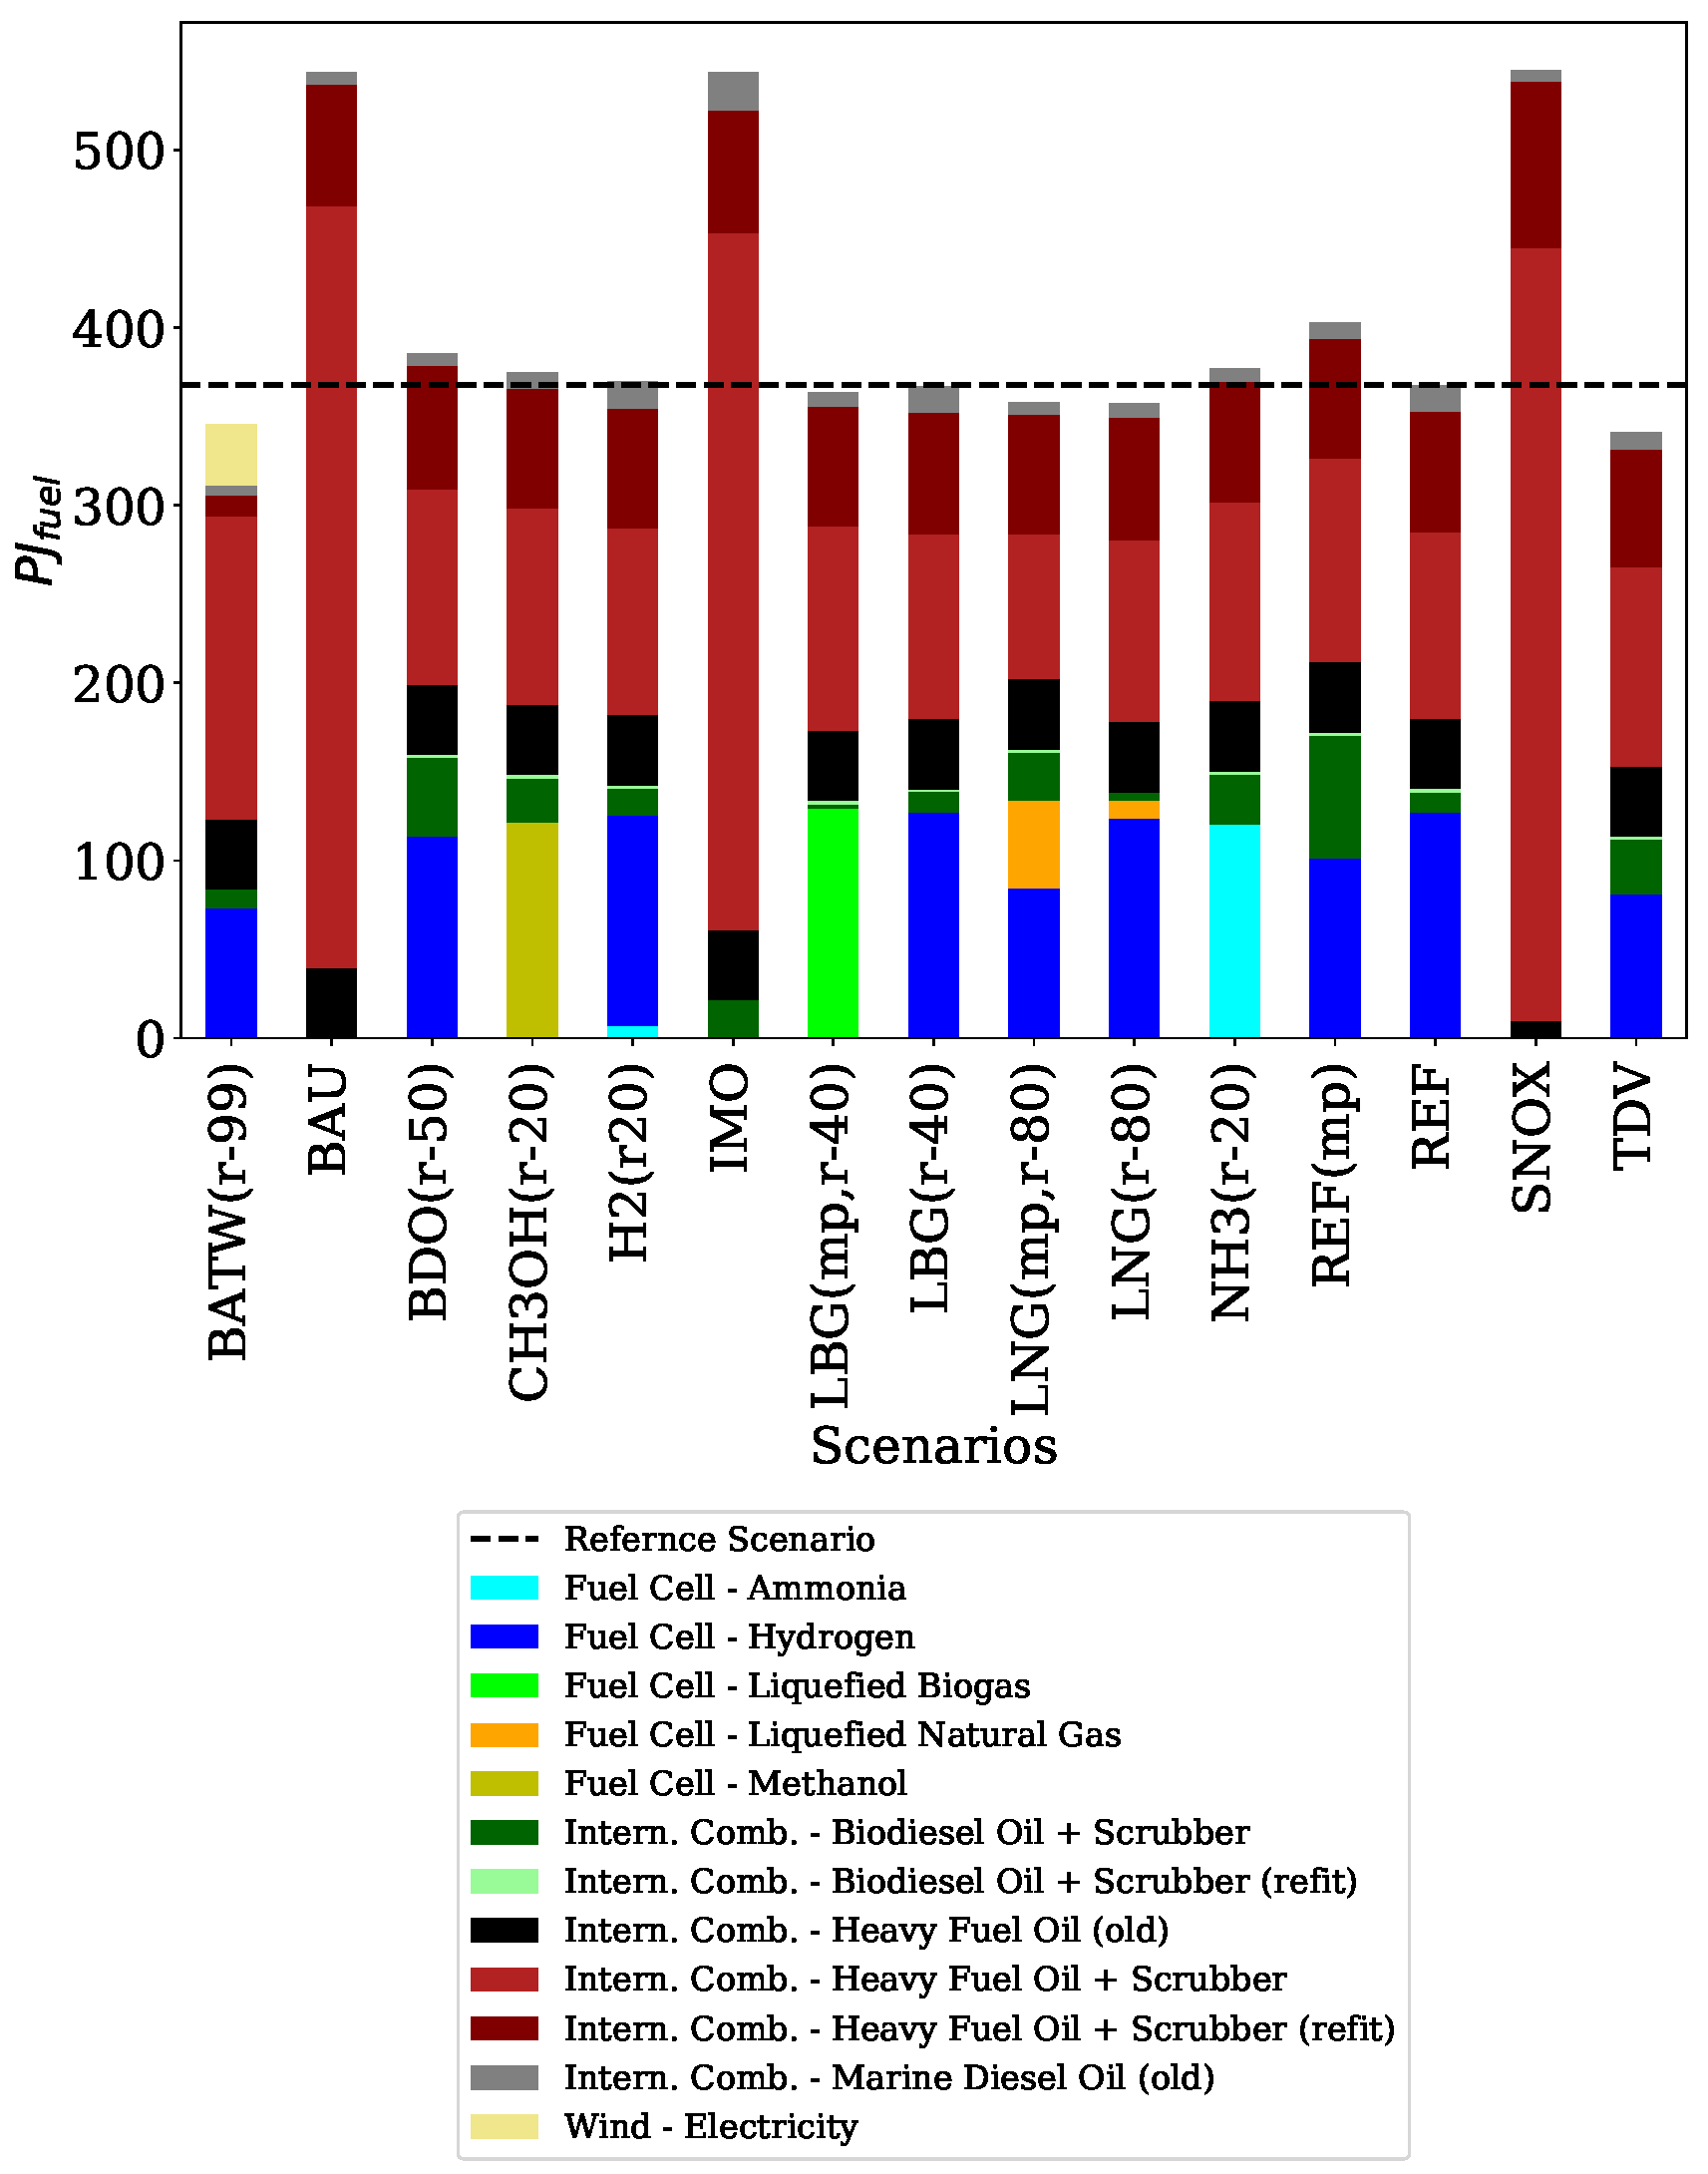
\includegraphics[width=.95\textwidth]{figures/AllFuelTotal.pdf}
    \label{fig:AllFuelTotal}
\end{minipage}
\begin{minipage}[t]{0.49\textwidth}
    \centering
    \captionsetup{justification=centering}
    \captionof{figure}{Fuel composition in 2050}
    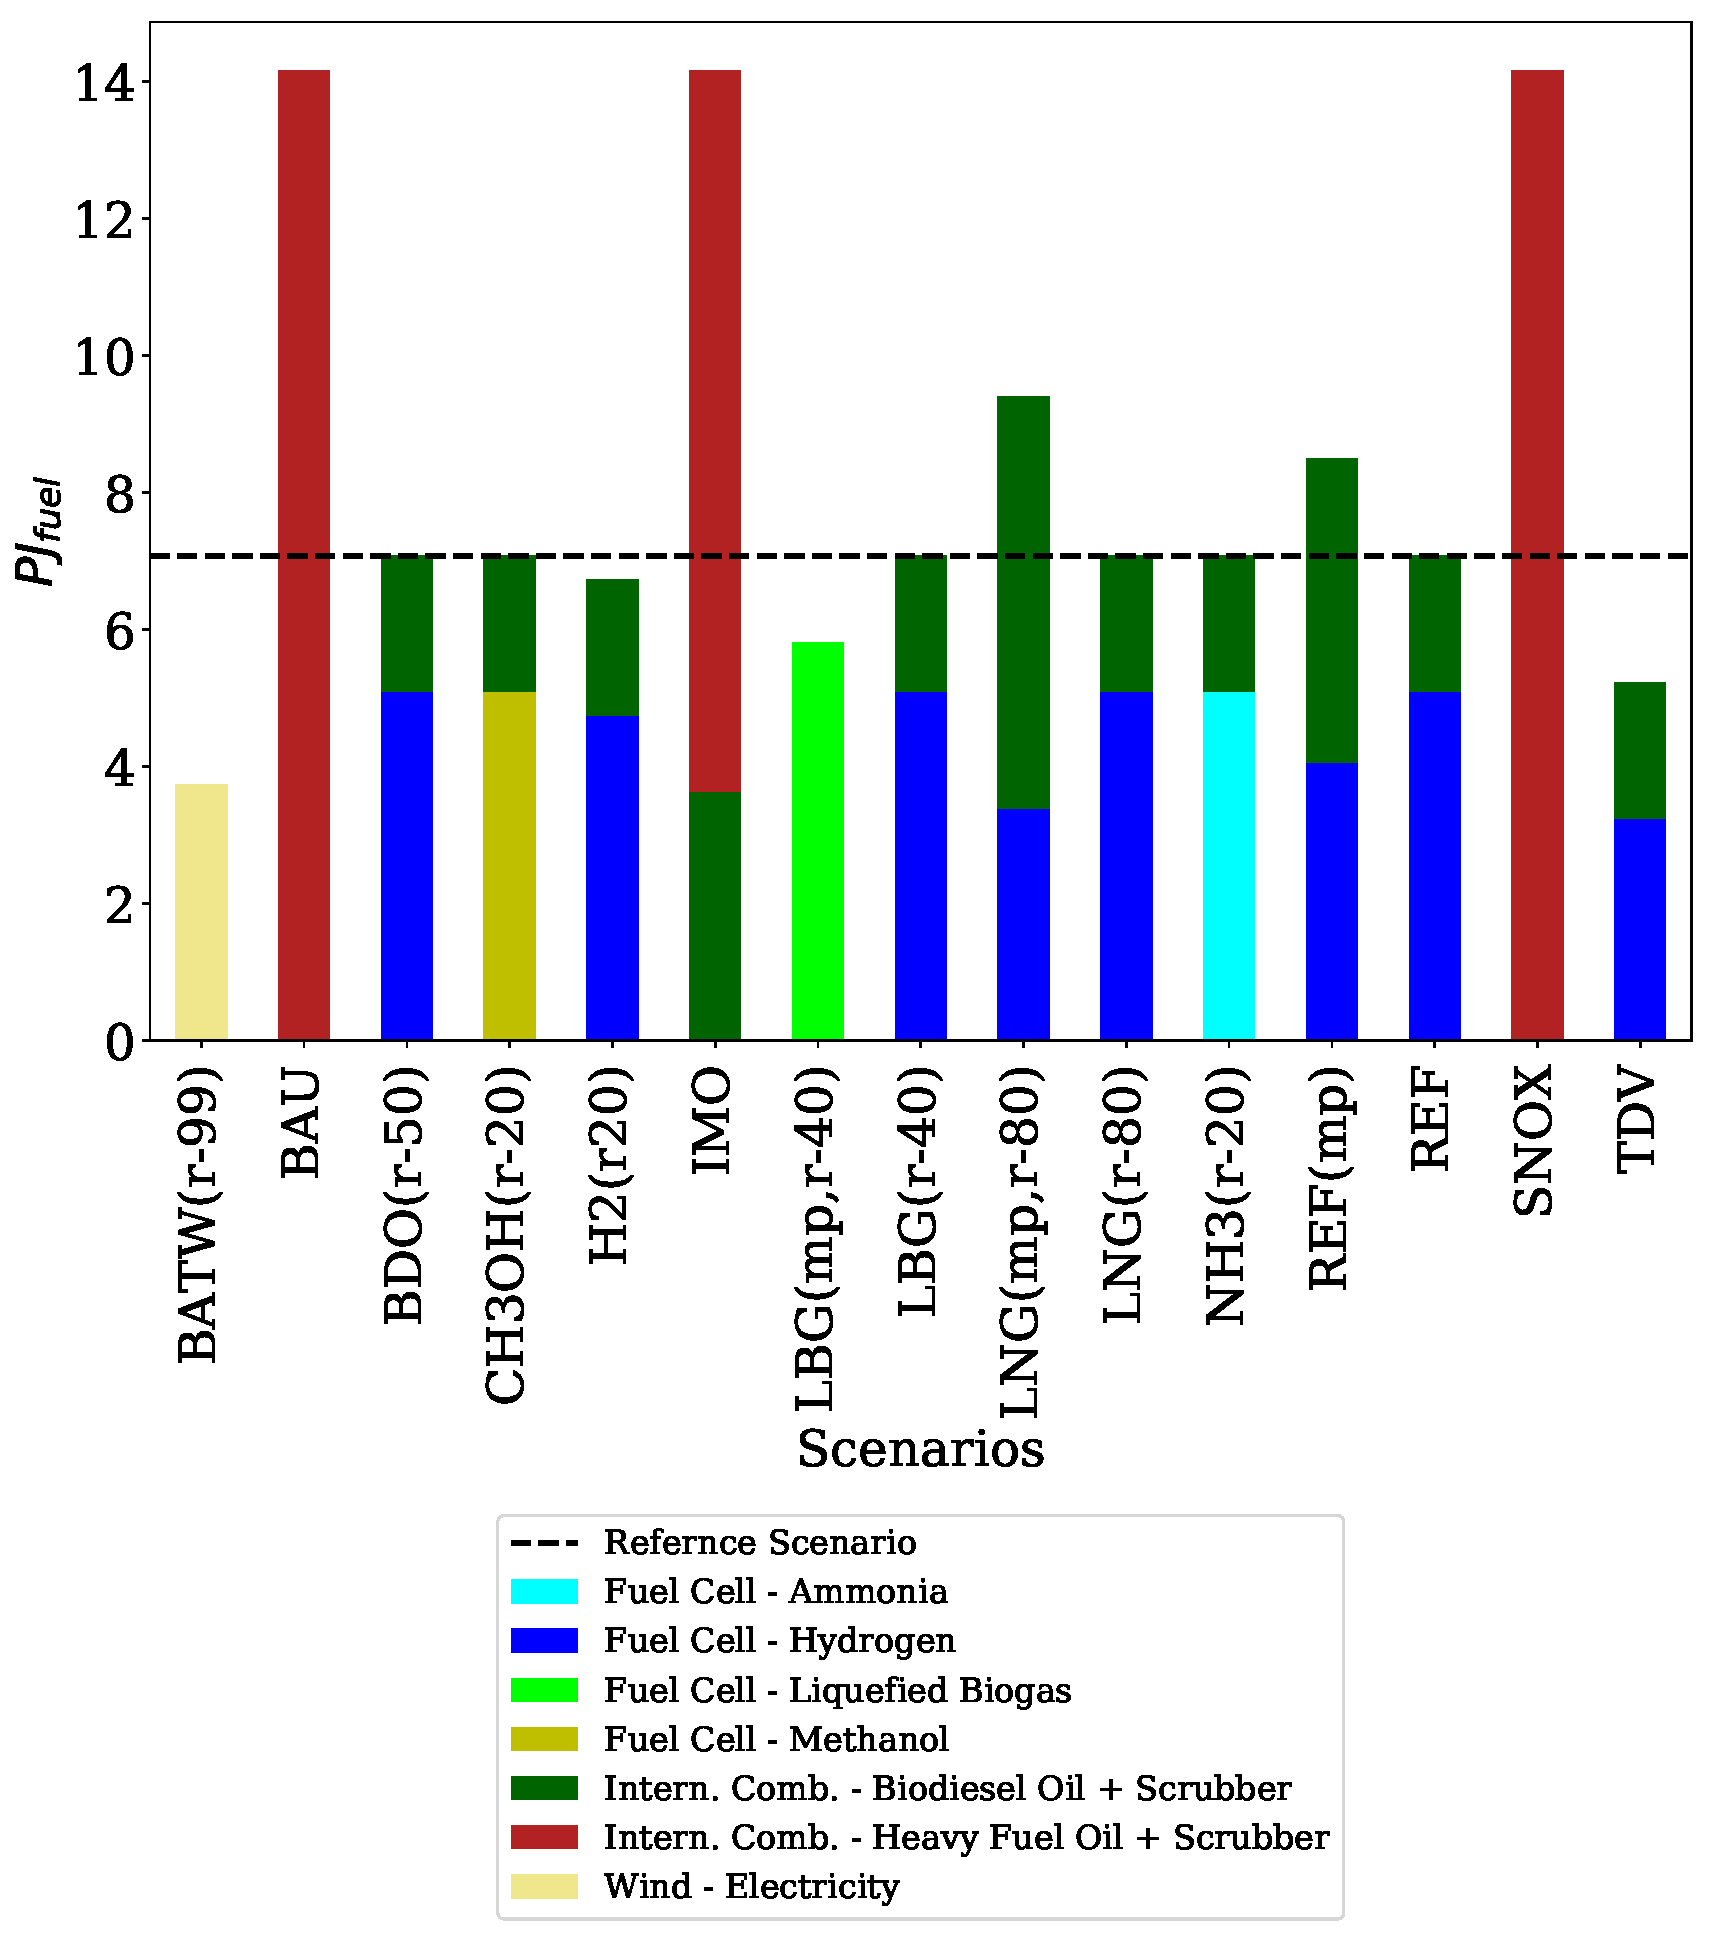
\includegraphics[width=.95\textwidth]{figures/AllFuel2050.pdf}
    \label{fig:AllFuel2050}
\end{minipage}\\[0.75cm]


% Compare all scenarios: Costs - not sure if there should be a figure - maybe rather include the full table of results

% Costs - resulting EURO/CO$_2$e
Derived from the cost differences for fuel, ship and infrastructure, a carbon price in the range of 350--450 \euro(2016)/ton CO$_2$e would be required for a renewable transition of the Danish shipping sector. \citep[p.197]{Raucci2017} reports similar prices of around 430 \$(2013)/ton CO$_2$ for a global transition.

% applicability of the model on other countries
% applicability of the findings for the world shipping
The model code and most of the data references and pre-processing can also be applied for other countries, especially Europe. However, since shipping has a global perspective, the case study for Denmark already gives a good indication of the fuel shares chosen for a cost-optimal path to carbon neutrality in 2050 for the worldwide shipping. Conditions for shipping are similar, the basic parameters, technology, fuel and infrastructure costs are considered as world prices rather than reflecting local particularities. This is also reflected and validated by the similar CO$_2$e-cost range compared to other, worldwide studies. 

% Why the mentioned costs are rather the upper end
Compared to other sectors like electricity and heat, these mitigation costs per ton CO$_2$e seem high, one has to consider several points. First, this is the upper bound of cost: Technologies considered are all applicable today, developments in other sectors applying similar fuel switch options could further influence costs, additional alternatives could evolve. Second, as shown in the demand reduction scenarios, any decrease in transport demand would save costs even beyond the proportional saving. This is due to not only fuel savings (proportional) but, also due to avoided investments in new ships (disproportionate). And third, refits and hybrid solutions have not been considered to a great extent in the model functionality and could further decrease costs and ease the shift to different fuels.


% Costs - what does that mean for the cargo cost
Transport costs in the BAU scenario amount to roughly 3 EUR2016 per ton cargo. For climate compatible pathways they are likely to more than double. With \cite[p.~50]{UNCTAD2015} reporting average transport costs of around 5 EUR per ton and including more detail, our results seem to be in an acceptably precise. Further, \cite[p.~55]{UNCTAD2015} states that transport costs in developed countries are equal to 7 \% of the cargo's import value. Under the assumption of an equal share in BAU, cargo import values for the climate compatible pathways would increase by 6 to 8 \%.

% Calculation:
% \begin{equation}
%     \text{Additional cost of cargo} = \frac{2\cdot3\frac{EUR}{t}}{\frac{3\frac{EUR}{t}}{7\%} - 3\frac{EUR}{t} + 2\cdot3\frac{EUR}{t}} - 7\%
% \end{equation}


% Co-benefits.
Thus, costs could get lower for the transition, but the question is also whether to talk about mitigation costs. Co-benefits like reduced air pollution have not been quantified on a monetary basis in the model and were thus not part of the optimisation. However, these could have essential health benefits, maybe even reaching mitigation gains instead of mitigation costs.

% Regulation / Recommendations
The necessary transition will not happen under current market conditions. Regulation is required urgently to bring shipping on the pathway to carbon neutrality in 2050, in line with the Paris Agreement. A carbon budget for shipping worldwide, broken down to countries is a viable option to consider. Additionally research money for alternative fuels and technologies, as well as solving crucial questions on security, infrastructure and methane leakage issues are important contributions to implement the transition to climate neutral shipping in 2050. 

% might be missing: strengths ad weaknesses of te model.
% Could also be added in the discussion: Important to model this in connection to the whole energy system, has effects!!

\section{Conclusion}
\label{sec:Conclusion}
% 250 words
% only draft until now!
The achievement of CO$_2$-neutrality in the shipping sector is of great importance for reaching the targets of the Paris Agreement. Although this goal is underrepresented in the current discussion, this study shows, that it is possible for the Danish part of international shipping to become CO$_2$-neutral until 2050 with existing technologies. Regarding fuels, hydrogen, methanol and ammonia are from a socio-economic cost perspective the most compatible. Due to high uncertainties regarding future cost developments and safety requirements (esp. ammonia), there is no clear winner. Regarding technologies, fuel cells are chosen for these fuel options, the decisive parameter being the higher fuel efficiency. Although LNG is the fuel option most prominently discussed as an alternative today, it would only have a short window of opportunity, mainly because of leakage problems of methane causing high greenhouse gas emissions as well as high fuel and technology costs. If this gaseous fuel is based on renewable sources, the so-called LBG can only play a role if methane leakage can be drastically reduced until 2050. The option of cargo-ships driven by a mixture of wind and electricity stored in batteries could not adequately be represented in the model setting. The evaluation of their role would need a further refinement of the calculations.
%Although additional conditions for the future application of fuel for shipping like safety issues or infrastructure decisions are not reflected in the model, ...
The presented modelling approach indicates that either strong regulative carbon budgets or a carbon price of 350--450 \euro/t~CO$_2$e would be required to induce the necessary changes for a carbon neutral Danish shipping in 2050. This would double today's average cargo transport costs. However, due to the low share of transport cost on the value of transported goods, the average transported good would only increase by 6 to 8 \%. This can be considered as the upper limit, since new fuel possibilities not reflected in this study might evolve.

\section*{References}

\bibliography{mybibfile}

\end{document}